\documentclass[10pt,twocolumn]{article}
\usepackage[utf8]{inputenc}

% Fix section numbering format - explicit control of how section numbers appear
\renewcommand{\thesubsection}{\thesection.\arabic{subsection}}
\usepackage{amsmath,amssymb}
\usepackage{graphicx}
\usepackage{xcolor}
\usepackage{tikz}
\usepackage{pgfplots}
\pgfplotsset{compat=1.18}
\usetikzlibrary{petri,positioning,arrows,automata,decorations.pathreplacing,shapes}

% For proper abstract formatting in two-column layout
\usepackage{abstract}
\usepackage{changepage}

% Improved URL and bibliography handling
\usepackage[hyphens,spaces,obeyspaces]{xurl}  % Better URL breaking

% Load hyperref with specific settings to fix section numbering in bookmarks
\usepackage[bookmarksnumbered,pdfstartview=FitH,hypertexnames=false]{hyperref}

% Configure hyperref for better URL breaking and appearance
\hypersetup{
    breaklinks=true,
    colorlinks=true,
    linkcolor=blue,
    urlcolor=blue,
    citecolor=blue,
    urlbordercolor={0 1 1},  % Cyan border around URLs (can remove if not needed)
    linkbordercolor=blue,    % Border color around links
    pdfborderstyle={/S/U/W 1} % Underline style for links (instead of border)
}

% Better URL breaking and formatting
\urlstyle{sf}  % Use sans-serif font for URLs
\def\UrlBreaks{%
  \do\a\do\b\do\c\do\d\do\e\do\f\do\g\do\h\do\i\do\j\do\k\do\l\do\m%
  \do\n\do\o\do\p\do\q\do\r\do\s\do\t\do\u\do\v\do\w\do\x\do\y\do\z%
  \do\A\do\B\do\C\do\D\do\E\do\F\do\G\do\H\do\I\do\J\do\K\do\L\do\M%
  \do\N\do\O\do\P\do\Q\do\R\do\S\do\T\do\U\do\V\do\W\do\X\do\Y\do\Z%
  \do0\do1\do2\do3\do4\do5\do6\do7\do8\do9\do.\do-\do_\do/\do!\do?\do\%
}
\usepackage{listings}

% Custom code listing style for smaller font and line breaks
\lstdefinestyle{gasingcode}{
  breaklines=true,
  basicstyle=\footnotesize\ttfamily,
  columns=fullflexible,
  keepspaces=true,
  frame=single,
  numbers=left,
  numberstyle=\tiny,
  xleftmargin=1.5em,
  xrightmargin=0.5em,
  aboveskip=0.5em,
  belowskip=0.5em
}

% Set default style for all listings
\lstset{style=gasingcode}
\usepackage{booktabs}
\usepackage{float}
\usepackage{enumitem}

% Simplest possible approach for watermark
\usepackage{rotating}
\usepackage{eso-pic}

% Direct watermark positioning in the left margin
\newcommand{\watermarktext}{arXiv:2025.12345v2 [cs.CL] \today}
\AddToShipoutPictureFG{%
  \AtPageCenter{%
    \put(-0.48\paperwidth+20pt,0){%
      \makebox(0,0)[c]{%
        \rotatebox{90}{%
          \textcolor{black!40}{\fontsize{18pt}{20pt}\selectfont\bfseries\watermarktext}%
        }%
      }%
    }%
  }%
}

% Watermark for draft version
\usepackage{draftwatermark}
\SetWatermarkText{DRAFT VERSION 0.1.133}
\SetWatermarkScale{0}
\SetWatermarkColor[gray]{0.85}

% Define our own styles for diagrams
\tikzset{
    operation/.style={
        rectangle,
        draw=black,
        thick,
        fill=blue!10,
        minimum height=1cm,
        minimum width=2.5cm,
        text centered
    }
}

% Load Spivak/Fong TikZ wiring diagram macros
% TikZ wiring diagram macros and styles from Spivak_Fong.tex (for use in other documents)
% Extracted for use in main.tex and figures/clock_with_display.tex

% TikZ libraries (make sure you load tikz and these libraries in your main doc)
\usetikzlibrary{
	cd,
	math,
	decorations.markings,
	decorations.pathreplacing,
	positioning,
	arrows.meta,
	circuits.logic.US,
	shapes,
	calc,
	fit,
	quotes}

% Macros
\newcommand{\tn}{\textnormal}
\newcommand{\inp}[1]{#1^{\tn{in}}}
\newcommand{\outp}[1]{#1^{\tn{out}}}
\newcommand{\upd}[1]{#1^{\tn{upd}}}
\newcommand{\rdt}[1]{#1^{\tn{rdt}}}

% Wiring diagram styles
\tikzset{
   oriented WD/.style={%everything after equals replaces "oriented WD" in key.
      every to/.style={out=0,in=180,draw},
      label/.style={
         font=\everymath\expandafter{\the\everymath\scriptstyle},
         inner sep=0pt,
         node distance=2pt and -2pt},
      semithick,
      node distance=1 and 1,
      decoration={markings, mark=at position \stringdecpos with \stringdec},
      ar/.style={postaction={decorate}},
      execute at begin picture={\tikzset{
         x=\bbx, y=\bby,
         every fit/.style={inner xsep=\bbx, inner ysep=\bby}}}
      },
   string decoration/.store in=\stringdec,
   string decoration={\arrow{stealth};},
   string decoration pos/.store in=\stringdecpos,
   string decoration pos=.7,
   bbx/.store in=\bbx,
   bbx = 1.5cm,
   bby/.store in=\bby,
   bby = 1.5ex,
   bb port sep/.store in=\bbportsep,
   bb port sep=1.5,
   bb port length/.store in=\bbportlen,
   bb port length=4pt,
   bb penetrate/.store in=\bbpenetrate,
   bb penetrate=0,
   bb min width/.store in=\bbminwidth,
   bb min width=1cm,
   bb rounded corners/.store in=\bbcorners,
   bb rounded corners=2pt,
   bb small/.style={bb port sep=1, bb port length=2.5pt, bbx=.4cm, bb min width=.4cm, bby=.7ex},
   bb medium/.style={bb port sep=1, bb port length=2.5pt, bbx=.4cm, bb min width=.4cm, bby=.9ex},
   bb/.code 2 args={%When you see this key, run the code below:
      \pgfmathsetlengthmacro{\bbheight}{\bbportsep * (max(#1,#2)+1) * \bby}
      \pgfkeysalso{draw,minimum height=\bbheight,minimum width=\bbminwidth,outer sep=0pt,
         rounded corners=\bbcorners,thick,
         prefix after command={\pgfextra{\let\fixname\tikzlastnode}},
         append after command={\pgfextra{\draw
            \ifnum #1=0{} \else foreach \i in {1,...,#1} {
               ($ (\fixname.north west)!{\i/(#1+1)}!(\fixname.south west) $)+( -\bbportlen,0)
               coordinate (\fixname_in\i) -- +(\bbpenetrate,0) coordinate (\fixname_in\i')}
            \fi
            %Define the endpoints of tickmarks
            \ifnum #2=0{} \else foreach \i in {1,...,#2} {
               ($ (\fixname.north east)!{\i/(#2+1)}!(\fixname.south east) $)+( -\bbpenetrate,0)
               coordinate (\fixname_out\i') -- +(\bbportlen,0) coordinate (\fixname_out\i)}
            \fi;
         }}}},
   bb name/.style={append after command={\pgfextra{\node[anchor=north] at (\fixname.north) {#1};}}}
}

% Additional unoriented WD styles (optional, but harmless)
\tikzset{
  unoriented WD/.style={
     every to/.style={draw},
     shorten <=-\penetration, shorten >=-\penetration,
     label distance=-2pt,
     thick,
     node distance=\spacing,
     execute at begin picture={\tikzset{
        x=\spacing, y=\spacing}}
     },
  pack size/.store in=\psize,
  pack size = 8pt,
  spacing/.store in=\spacing,
  spacing = 8pt,
  link size/.store in=\lsize,
  link size = 2pt,
  penetration/.store in=\penetration,
  penetration = 2pt,
  pack color/.store in=\pcolor,
  pack color = blue,
  pack inside color/.store in=\picolor,
  pack inside color=blue!20,
  pack outside color/.store in=\pocolor,
  pack outside color=blue!50!black,
  surround sep/.store in=\ssep,
  surround sep=8pt,
  link/.style={
     circle, 
     draw=black, 
     fill=black,
     inner sep=0pt, 
     minimum size=\lsize
  },
  pack/.style={
     circle, 
     draw = \pocolor, 
     fill = \picolor,
     inner sep = .25*\psize,
     minimum size = \psize
  },
  outer pack/.style={
     ellipse, 
     draw,
     inner sep=\ssep,
     color=\pocolor,
  },
  intermediate pack/.style={
     ellipse,
     dashed, 
     draw,
     inner sep=\ssep,
     color=\pocolor,
  },
}


% Load arxiv.sty LAST to override previous settings
\usepackage{arxiv}

% Custom title settings - set format for arXiv style
\renewcommand{\shorttitle}{GASing Arithmetic}
\renewcommand{\undertitle}{A Preprint}
\renewcommand{\headeright}{arXiv:2025.12345v1}

% Set document title and author
\title{Pattern-Aware, Addition-Based Computation for\\Next-Generation AI}
\author{Yohanes Surya\\AI Toba Project, IT Del\\Toba, Indonesia\\yohanes.surya@del.ac.id}

% Use simple header/footer settings
\pagestyle{fancy}
\fancyhf{} % Clear all header/footer fields
\renewcommand{\headrulewidth}{0.4pt}
\fancyheadoffset{0pt}
\rhead{\scshape \footnotesize \headeright}
\chead{\shorttitle}
\cfoot{\thepage}

\begin{document}

% Enable page numbering
\pagestyle{plain}
\pagenumbering{arabic}

% Set column separation for better readability
\setlength{\columnsep}{0.5in}

% Temporarily switch to onecolumn for title and abstract
\onecolumn

% Create a more journal-like title
\begin{center}
\vspace*{-2cm}
\rule{\textwidth}{0.4pt}
\vspace{0.1cm}
{\LARGE\textbf{Pattern-Aware, Addition-Based Computation for\\Next-Generation AI}}\\
\vspace{0.5cm}
\rule{\textwidth}{0.4pt}
\vspace{0.5cm}
{\normalsize\textbf{Yohanes Surya}}\\
{\small AI Toba Project, IT Del}\\
{\small Toba, Indonesia}\\
{\small yohanes.surya@del.ac.id}\\
\vspace{0.3cm}
{\small May 27, 2025}\\
\vspace{1cm}
\end{center}

% Abstract with full text width to match document width
\begin{center}
{\large\textbf{Abstract}}
\end{center}
\vspace{-0.3cm}
The \textbf{\textit{GASing Arithmetic}} method introduces a foundational paradigm for numerical computation at the intersection of human cognition, cultural mathematics, and artificial intelligence. Drawing inspiration from Eglash's work in \textbf{\textit{Ethno Arithmetic}} and fractal patterns in indigenous knowledge systems, GASing demonstrates how culturally-grounded mathematical insights can inform modern computational frameworks. In an era where AI systems increasingly shape and augment human reasoning, there is a critical need for computational approaches that are not only transparent and interpretable but also capable of aligning with fundamental cognitive patterns across diverse cultural contexts. GASing addresses this challenge through the \textbf{progressive application of functions} and \textbf{digit-wise systems as cell-like modules}, establishing \textbf{addition as the universal meta-operator}—the cornerstone of a minimized operational vocabulary from which all arithmetic logic can be systematically constructed, analyzed, and verified. 

This approach leverages the inherent combinatorial patterns in self-similar systems to better compress unnecessary computational efforts. Through digit-wise processing and pattern recognition, GASing enables explicit quantification of computational effort and resource usage, bridging symbolic and neural approaches while supporting robust provenance tracking. The method's cell-like modular architecture, inspired by the fractal patterns found in traditional Indonesian design and other indigenous knowledge systems, allows for efficient information processing by breaking down complex operations into manageable, recombinable units. This unified approach has been successfully implemented in Indonesia's national education program, reaching millions of students and demonstrating how culturally-informed knowledge exchange protocols can be continuously improved at scale. Our findings demonstrate that GASing is not only a mathematically rigorous and pedagogically effective framework, but also a culturally-grounded substrate for interpretable, trustworthy, and resource-efficient AI—laying the groundwork for a unified theory of learning rooted in both universal mathematical principles and diverse cultural expressions of mathematical thinking.

\vspace{1cm}

% Return to two-column layout
\twocolumn

\section{Introduction}
% This LaTeX document is prepared using the arXiv style guidelines
% https://arxiv.org/help/submit_tex

\sectionheader{Introduction}

We propose a novel synthesis of Petri Nets and tensor algebra, arguing that Petri Nets can leverage the mathematical formalism of tensors to represent topologically related operands and their interactions. Drawing on David Spivak’s theory of polynomial functors, we introduce the concept of a Tensorized Petri Net, where each element can act simultaneously as an operand and an operator. We illustrate this framework using digit-wise arithmetic, showing how it enables compositional, interpretable, and parallelizable symbolic computation.

Petri Nets are a foundational tool for modeling distributed and concurrent systems, providing a graphical and mathematical language for representing state, transitions, and resource flow. Traditionally, Petri Nets are used to model discrete events and token flows, but recent advances in neural-symbolic computation and category theory suggest new ways to enrich their expressive power.

In this work, we argue that Petri Nets can be “tensorized”—that is, their places, transitions, and token flows can be represented and manipulated using tensor algebra. Tensors, as multi-dimensional arrays, provide a powerful language for encoding the state of complex systems, capturing not only the presence of tokens but also their relationships and interactions across multiple dimensions. By mapping Petri Net components to tensor indices and operations, we can efficiently model the evolution of distributed systems, exploit parallel computation, and reveal underlying topological structures. This approach is particularly advantageous for systems where locality, adjacency, or compositionality play a central role, such as in digit-wise arithmetic or spatially structured processes.

Furthermore, by leveraging David Spivak’s ideas on polynomial functors, we can treat every element in the net as both an operand and an operator, capturing higher-order compositionality and self-similarity. This categorical perspective allows us to formalize the ways in which Petri Nets and tensors interact, supporting modular design and scalable reasoning.

The main components of Petri Nets include:
\begin{itemize}
    \item Places (represented as circles)
    \item Transitions (represented as rectangles)
    \item Arcs (directed edges connecting places to transitions or transitions to places)
    \item Tokens (represented as dots within places)
\end{itemize}

In this paper, we explore the application of Petri Nets to model [specific system or process], with a focus on [specific aspect or property]. % In the section where you list contributions:

Our contributions include:
\begin{itemize}[leftmargin=*,align=left]
    \item \textbf{Contribution 1:} A novel approach to modeling concurrent processes using Petri Nets.
    \item \textbf{Contribution 2:} Analysis of deadlock properties in the context of resource allocation.
    \item \textbf{Contribution 3:} Implementation and evaluation of the proposed model using simulation.
\end{itemize}

// Remove the duplicate contributions list
% The main contributions of this work include:
% \begin{IEEEkeywords}
% Petri Nets, TikZ, formal modeling, concurrent systems
% \end{IEEEkeywords}
% \begin{itemize}[leftmargin=*,align=left,widest=Contribution 3]
%   \item \textbf{Contribution 1:} Description of your first contribution...
%   \item \textbf{Contribution 2:} Description of your second contribution...
%   \item \textbf{Contribution 3:} Description of your third contribution...
% \end{itemize}

The remainder of this paper is organized as follows: Section \ref{sec:background} provides background information and related work. Section \ref{sec:methodology} describes our methodology and the proposed Petri Net model. Section \ref{sec:results} presents the results and analysis. Finally, Section \ref{sec:conclusion} concludes the paper and discusses future work.

\section{Foundational Principles}
The GASing method is built upon several coherent principles designed to simplify arithmetic into a minimal set of understandable and computationally efficient operations. These principles collectively support the goal of grounding all arithmetic in addition, thereby clarifying resource consumption and enhancing the interpretability of reasoning processes.
\paragraph{The Digit-Wise Processing Paradigm}

At its core, GASing employs a digit-wise processing approach that, instead of merely breaking numbers into fixed constituent digits, flexibly defines the boundaries of arithmetic operations by utilizing the topological properties of Carry and Borrow propagations between adjacent numerical segments (or 'digits'). The granularity of these segments can be dynamically determined to optimize arithmetic calculation efficiency, particularly leveraging the observation that operations become highly efficient when all unique combinations of numerical values within these segments can be assessed \emph{a priori}. This refined digit-wise paradigm is fundamental to minimizing the complexity of the operational vocabulary. Instead of treating numbers as holistic entities requiring a potentially tedious array of complex operations, GASing focuses on manipulating these individual segments using a very limited set of rules, primarily those governing the foundational principles of addition applied at the segment level. This approach aligns with both human cognitive abilities and computational architecture:

- \textbf{Human Cognition}: By processing operations at the level of these flexibly defined numerical segments (which can be as small as single digits), GASing leverages established neural pathways for simpler operations (Dehaene, 2011). This modular, segment-based processing keeps the cognitive load for each step manageable, making the system intuitive and easier for human users to verify, even as the definition of a 'segment' adapts for efficiency.
- \textbf{Computational Architecture}: This segment-wise processing, where segments can be optimized for computational efficiency (e.g., to fit register sizes or leverage pre-computed lookup tables for segment-level operations), maps effectively to modern processor capabilities. Reducing operations to their simplest form at the segment level (e.g., segment addition and inter-segment carry/borrow) allows for granular understanding, control of computational resources, and potential for optimized hardware implementations.

This fine-grained processing is key to building complex operations from the simplest possible base, ensuring that the entire system remains transparent and its resource demands predictable.
\paragraph{Modular Operation Design: A Minimal Vocabulary Anchored in Addition}

GASing builds all arithmetic operations as modular extensions of one another, with \textbf{addition, applied at the level of flexibly defined numerical segments, serving as the single, foundational operator}. This hierarchical construction, leveraging the segment-wise processing described earlier, is central to achieving a minimal operational vocabulary and directly impacts the assessment of resource consumption:

1.  \textbf{Segment-wise Addition} serves as the foundational, irreducible operation. All other arithmetic operations are defined in terms of sequences or transformations of this fundamental segment-wise addition, including the management of carry and borrow propagations between segments.
2.  \textbf{Multiplication} is constructed as specialized, repeated segment-wise addition. The process involves systematic application of segment-level additions and accumulation of partial results, explicitly defining multiplication's resource cost in terms of the underlying additive operations on segments.
3.  \textbf{Subtraction} is implemented as segment-wise addition using complementary segment values (e.g., employing ten's complement for decimal segments or two's complement for binary segments). This reframes subtraction entirely within the additive framework at the segment level, maintaining the minimal operational vocabulary.
4.  \textbf{Division} is approached through repeated segment-wise subtraction (which, as noted, is itself addition-based) with optimizations that can leverage pattern recognition across segments. Its complexity and resource use are, therefore, also traceable back to the fundamental segment-wise addition operations.

This modularity, centered on segment-wise addition, creates a coherent and parsimonious framework. Mastery of segment-wise addition directly facilitates the understanding and implementation of all other operations. More importantly, it means that the entire arithmetic system can be analyzed, and its resource consumption (both cognitive and computational) can be estimated based on the number and type of segment-wise addition-equivalent steps involved. This contrasts sharply with systems where each operator might be a black box with unique, opaque resource demands, and it aligns with the goal of transparently assessing computational effort by reducing all operations to a common, addition-based denominator at a flexible granularity.
\paragraph{Lookup Tables and Pattern Recognition: Optimizing the Core Operator}

Central to the GASing method is the use of precomputed lookup tables for basic operations, \textbf{particularly for single-digit addition and its immediate consequences (like carry generation)}. These tables are not an expansion of the operational vocabulary but rather an optimization strategy for the core addition operator:

-   \textbf{Reduce Cognitive and Computational Load}: By pre-calculating and storing the results of all possible single-digit additions (e.g., 0+0 through 9+9), the need for real-time calculation of these base operations is eliminated. This directly speeds up the execution of the foundational operator.
-   \textbf{Enable Pattern Recognition}: Consistent use of lookup tables for the core additive step allows for the easier identification of recurring patterns across multiple calculations. This can lead to higher-level optimizations and a better understanding of the computational structure of a problem, all while still operating within an addition-centric framework.
-   \textbf{Analogous to Caching}: These tables function similarly to CPU cache mechanisms or memoization in computing systems, storing frequently accessed results to avoid redundant computation. This makes the core addition process highly efficient.

By optimizing the execution of the single core operator (addition) through lookup tables, GASing ensures that the minimal vocabulary does not come at the cost of prohibitive inefficiency for elementary steps. This focus on optimizing the fundamental building block is crucial for the scalability and practicality of the approach, ensuring that even complex reasoning built from these simple steps remains manageable in terms of resource consumption.


\section{GASing Implementation and Algorithms}
It is well known that certain primitives such as the NAND gate or the MOV instruction are considered the Universal Components in all Turing Complete decision machines. While these theoretical universality results are fundamental to computing, this article will focus specifically on how the addition operator can be adaptively executed based on available computing resources, serving as a practical foundation for higher-level reasoning. Moreover, efficient adders at the integrated circuit level, such as the Brent-Kung Adder, have proven to be highly efficient for addition operations in hardware implementations. However, based on different value pairs or value collections, there are still certain cases of arithmetic operations that could be executed with even fewer computing resources through pattern recognition and specialized implementations. These optimization opportunities, particularly for patterns like all-nines, power-of-ten, or sparse number representations, are the primary focus of this article and represent a complementary approach to hardware-level optimizations.
\paragraph{Addition Algorithm as a Functorial Petri Net}

The GASing addition algorithm processes numbers from left to right (most significant digit to least significant), a departure from the traditional right-to-left approach. This design choice is deliberate and offers several advantages rooted in computational efficiency and cognitive alignment, particularly when considering the broader goals of the GASing framework to minimize operational vocabulary and optimize resource consumption.
\paragraph{Multi-Digit Numbers as Interconnected Automata}

A novel way to conceptualize the GASing approach is through the lens of \textbf{Functorial Petri Nets} (\textbf{\textit{Functorial Petri Net}}), where each digit in a multi-digit number functions as a semi-autonomous cell within a larger network of computational agents. Under this framing:


\noindent\textbf{\textbf{Digit Positions as Petri Net Places}:} Each digit position in a multi-digit number corresponds to a discrete place in a Petri Net, capable of holding tokens that represent both the current digit value and potential carry/borrow states.



\noindent\textbf{\textbf{Arithmetic Operations as Transitions}:} The fundamental arithmetic operations (particularly addition) manifest as transitions in the Petri Net that consume tokens from input places (operand digits) and produce tokens in output places (result digits and carries).



\noindent\textbf{\textbf{Carry/Borrow as Message Propagation}:} The carry and borrow mechanisms essential to multi-digit arithmetic represent a formalized message-passing protocol between adjacent digit places. When a digit operation results in a value exceeding the base (e.g., 9+4=13 in decimal), a carry token is generated and propagated to the next significant digit place—a perfect example of resource-aware token flow characteristic of Petri Nets.



\noindent\textbf{\textbf{Compositionality Through Functors}:} The functorial nature of this representation ensures that the compositional structure of arithmetic operations is preserved across different levels of abstraction. This means that complex arithmetic sequences can be formally derived from compositions of simpler operations while maintaining their algebraic properties.


This Petri Net interpretation yields powerful insights into the GASing method's efficiency advantages:


\noindent\textbf{\textbf{Concurrency Potential}:} By analyzing the dependency structure between digit places, we can identify opportunities for concurrent processing. Digits not affected by carry chains can be computed independently, enabling parallelism.



\noindent\textbf{\textbf{Adaptive Segmentation Through Net Morphisms}:} The functorial properties allow us to define morphisms between different Petri Net configurations, formalizing how digit segments can be dynamically merged or split to optimize computational efficiency. These morphisms preserve the essential algebraic structure while enabling resource-adaptive execution.



\noindent\textbf{\textbf{Pattern Recognition as Specialized Transitions}:} Recurring patterns in digit configurations (such as all-nines or power-of-ten values) can be modeled as specialized transitions that bypass individual digit-by-digit processing, offering substantial performance benefits.


The integration of GASing and Functorial Petri Nets reveals arithmetic as fundamentally a \textbf{distributed, asynchronous computation process}, where each digit place operates with relative autonomy yet remains coordinated through precisely defined message passing protocols. This perspective not only provides a rigorous mathematical foundation for the GASing method but also suggests novel optimization strategies derived from Petri Net theory's rich analytical tools.

A key principle underpinning this algorithm is its explicit leverage of \textbf{n-ary arithmetic}. The algorithm is designed to be agnostic to the base of the numerical segments being processed. Whether the system operates in binary, tertiary, decimal, hexadecimal, or any other base (n-ary), the core logic of left-to-right processing with carry propagation remains consistent. This flexibility allows the system to adapt the granularity of its operations (i.e., the 'digit' size or segment length) to best fit resource consumption optimization schemes. For instance, the segment size can be chosen to align with the cache line size of a processor or the optimal block size for memory access, thereby minimizing latency and maximizing throughput for pre-calculated and stored intermediate results. \textbf{Critically, this optimization is specifically tailored to the resource requirements of the underlying hardware architecture}, enabling significant performance improvements when frequently-used digit pairs are identified and cached in lookup tables that match the machine's memory hierarchy.

This adaptability is crucial for applying GASing principles to complex reasoning activities, potentially even those embedded within advanced AI architectures like the \textbf{Sparse Autoencoders (SAEs)} described in the "Scaling MonoSemanticity" paper. SAEs aim to decompose complex model activations into a sparse set of interpretable, monosemantic features. In essence, an SAE learns a large dictionary of these features, where only a small subset is active for any given input. This learned dictionary of features in an SAE can be seen as analogous to a highly optimized, distributed lookup table within the GASing framework. 

The GASing addition algorithm, by being designed for flexible n-ary arithmetic and optimized segment processing, aligns well with such architectures. If the 'features' learned by an SAE can be mapped to or interact with the numerical segments processed by GASing, then the pre-calculated operations and lookup tables inherent in GASing could significantly enhance the efficiency and interpretability of these SAEs. The left-to-right processing allows for incremental computation and potential early termination if an approximate result suffices, which can be beneficial in resource-constrained environments or when dealing with the vast feature spaces of SAEs. Furthermore, by designing arithmetic operations that can be efficiently cached and retrieved, GASing can support the rapid activation and combination of these 'semantic features' in an SAE, effectively making the SAE a powerful, dynamic dictionary that GASing can interact with for reasoning tasks.

\textbf{The algorithm can dynamically accelerate computation when known digit pairs or patterns are detected}, adjusting its execution strategy based on the specific machine architecture in use. For example, performance can be dramatically improved (as demonstrated in our benchmarks showing up to 10x+ speedups for certain patterns) when retrieving content from optimally-structured lookup tables that match the CPU's cache hierarchy, memory access patterns, or SIMD capabilities. By incorporating fine-grained resource accounting at the level of the most primitive operation—addition—this approach provides the foundational mechanism for resource attribution and optimization in higher-level reasoning activities. This systematic accounting of computational resources, beginning at the elemental operation level, creates a transparent chain of resource utilization that extends seamlessly to complex symbolic processing, verification chains, and formal reasoning frameworks. The adaptive approach allows the algorithm to automatically exploit architectural features such as cache line prefetching, branch prediction, and specialized arithmetic units, delivering optimal performance across diverse computing environments without requiring manual tuning or specialized implementations.



\begin{figure}[H]
  \centering
  \includegraphics[width=\linewidth]{images/gasing\_addition\_single\_digit.png}
  \caption{GASing single-digit addition}
  \label{fig:gasingadditionsingledigit}
\end{figure}



This left-to-right, n-ary adaptable processing allows for:

\noindent\textbf{\textbf{Flexible Resource Optimization:} } Tailoring segment size (n-ary base) to hardware (cache, memory) or task demands.


\noindent\textbf{\textbf{Alignment with Human Cognition:} } Processing information sequentially, similar to reading.


\noindent\textbf{\textbf{Potential for Parallelization:} } Independent processing of segments once carries are managed.


\noindent\textbf{\textbf{Integration with Learned Representations:} } Provides a computational backend for systems like SAEs, where pre-calculated arithmetic on features (analogous to dictionary lookups) can speed up reasoning.


\noindent\textbf{\textbf{Early Termination for Approximations:} } Useful in iterative reasoning processes or when full precision is not immediately required.


By structuring the addition algorithm this way, GASing aims to provide a foundational arithmetic layer that is not only efficient in isolation but also highly compatible with modern AI architectures that rely on learned dictionaries and feature-based representations, such as Sparse Autoencoders.
\paragraph{Multiplication Algorithm}

The GASing multiplication algorithm fundamentally extends the principles of the GASing addition operator, reframing multiplication as a systematic process of repeated, structured addition. It conceptualizes the multiplication of two numbers as the summation of partial products arranged in a grid-like structure. This approach not only maintains the core philosophy of minimizing operational vocabulary by grounding operations in addition but also enhances clarity and traceability.

Each cell in the conceptual grid represents the product of two individual digits (or segments, in n-ary arithmetic), which can be pre-calculated or retrieved from lookup tables, similar to single-digit additions. The core of the multiplication process then becomes the systematic summation of these grid values, column by column (or diagonal by diagonal, depending on the specific grid layout), applying the GASing addition algorithm (including its left-to-right carry propagation) to these intermediate sums. This effectively transforms multiplication into a series of additions, organized spatially by the grid.

The following diagram illustrates this grid-based summation concept:


\begin{figure}[H]
  \centering
  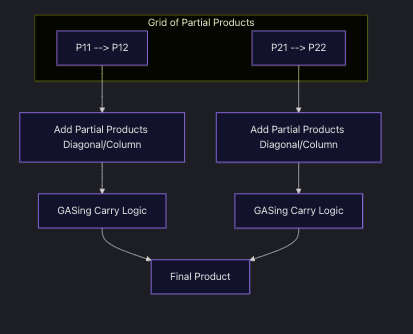
\includegraphics[width=\linewidth]{images/GridBasedMultiplication.png}
  \caption{Grid Based Multiplication}
  \label{fig:gridbasedmultiplication}
\end{figure}


The grid-based approach, when viewed as a structured application of the GASing addition algorithm, facilitates:


\noindent\textbf{\textbf{Clear Visualization}:} The multiplication process is broken down into a visible grid of elementary products (which are themselves results of lookup or minimal computation) and subsequent additions.


\noindent\textbf{\textbf{Systematic Carry Handling}:} Carries generated during the summation of grid elements are managed by the underlying GASing addition logic, ensuring consistency.


\noindent\textbf{\textbf{Reinforcement of Additive Core}:} Emphasizes that multiplication is not a fundamentally new operation but an organized, scaled-up application of addition.


\noindent\textbf{\textbf{Identification of Patterns}:} The structured grid can reveal patterns in partial products, which can be leveraged for optimization, especially when combined with n-ary segment processing and lookup tables for segment products.


By treating multiplication as an extension of addition via a grid, GASing maintains its commitment to a minimal operational vocabulary and enhances the interpretability of more complex arithmetic by tracing it back to foundational additive steps.
\paragraph{Subtraction and Division: Extending Addition Further}

Consistent with GASing's core tenet of a minimal operational vocabulary, both subtraction and division are conceptualized and implemented as extensions of the foundational GASing addition algorithm.
\paragraph{Subtraction as Complemented Addition}

Subtraction in GASing is performed by adding the complement of the subtrahend. For a given base (e.g., decimal or binary), the n's complement (e.g., ten's complement or two's complement) of the subtrahend is calculated and then added to the minuend using the \texttt{$GASing\_{Addition}$} algorithm. This reframes subtraction entirely as an additive process, reinforcing the minimal operator set.


\noindent\textbf{\textbf{N's Complement:} } The n's complement of a number \texttt{b} with \texttt{k} digits in base \texttt{n} is \texttt{$(n^{k} - b)$}. A common way to compute this is by finding the (n-1)'s complement (subtracting each digit from \texttt{n-1}) and then adding 1 to the result.


\noindent\textbf{\textbf{Process:} } To compute \texttt{a - b}, GASing calculates \texttt{a + (n's complement of b)}. If an overflow carry occurs from the most significant digit, it is typically discarded (in fixed-width representations), and the remaining result is the positive difference. If no overflow occurs, the result is negative, and its true magnitude is the n's complement of the sum, often flagged appropriately.





\noindent --

\paragraph{Division as Repeated Subtraction (Repeated Complemented Addition)}

Division, in its most fundamental GASing form, is conceptualized as repeated subtraction. Given that subtraction itself is an additive operation (using complements), division becomes a higher-order construct built upon layers of addition.


\noindent\textbf{\textbf{Process:} } To compute \texttt{a / b}, GASing repeatedly subtracts \texttt{b} (the divisor) from \texttt{a} (the dividend) using the \texttt{$GASing\_{Subtraction}$} method. The number of successful subtractions before \texttt{a} becomes less than \texttt{b} (or zero) constitutes the quotient. The final value of \texttt{a} after these subtractions is the remainder.


\noindent\textbf{\textbf{Optimization:} } While simple repeated subtraction can be inefficient, GASing allows for optimizations. These can include subtracting multiples of \texttt{b} (e.g., \texttt{10\emph{b}, \texttt{100}b}), similar to long division, or leveraging pattern recognition to estimate parts of the quotient more quickly. However, even these optimized steps are ultimately resolved through sequences of the core \texttt{$GASing\_{Subtraction}$} (and therefore \texttt{$GASing\_{Addition}$}) operations.



\noindent --


By defining subtraction and division in terms of addition, GASing ensures that the entire arithmetic framework remains anchored to a single, fundamental operation. This not only simplifies the conceptual model but also provides a consistent basis for analyzing computational resource consumption, as all operations can be broken down into equivalent additive steps.


\section{Performance Benchmarking}
Our current benchmarking evaluates how different GASing implementations handle specific mathematical sequences, such as:

- Fibonacci numbers
- Factorial values
- Powers of 2
- Prime numbers
- Repdigits (numbers with repeated digits)
- Alternating digit patterns

While these tests reveal that certain GASing implementations show clear advantages for specific patterns (e.g., the optimized C implementation excels at repdigit sequences due to efficient carry pattern recognition), the broader significance lies in the future direction of this benchmarking.

The following diagrams show the performance of different GASing implementations on digit-wise arithmetic operations based on String manipulation.

\begin{figure}[H]
  \centering
  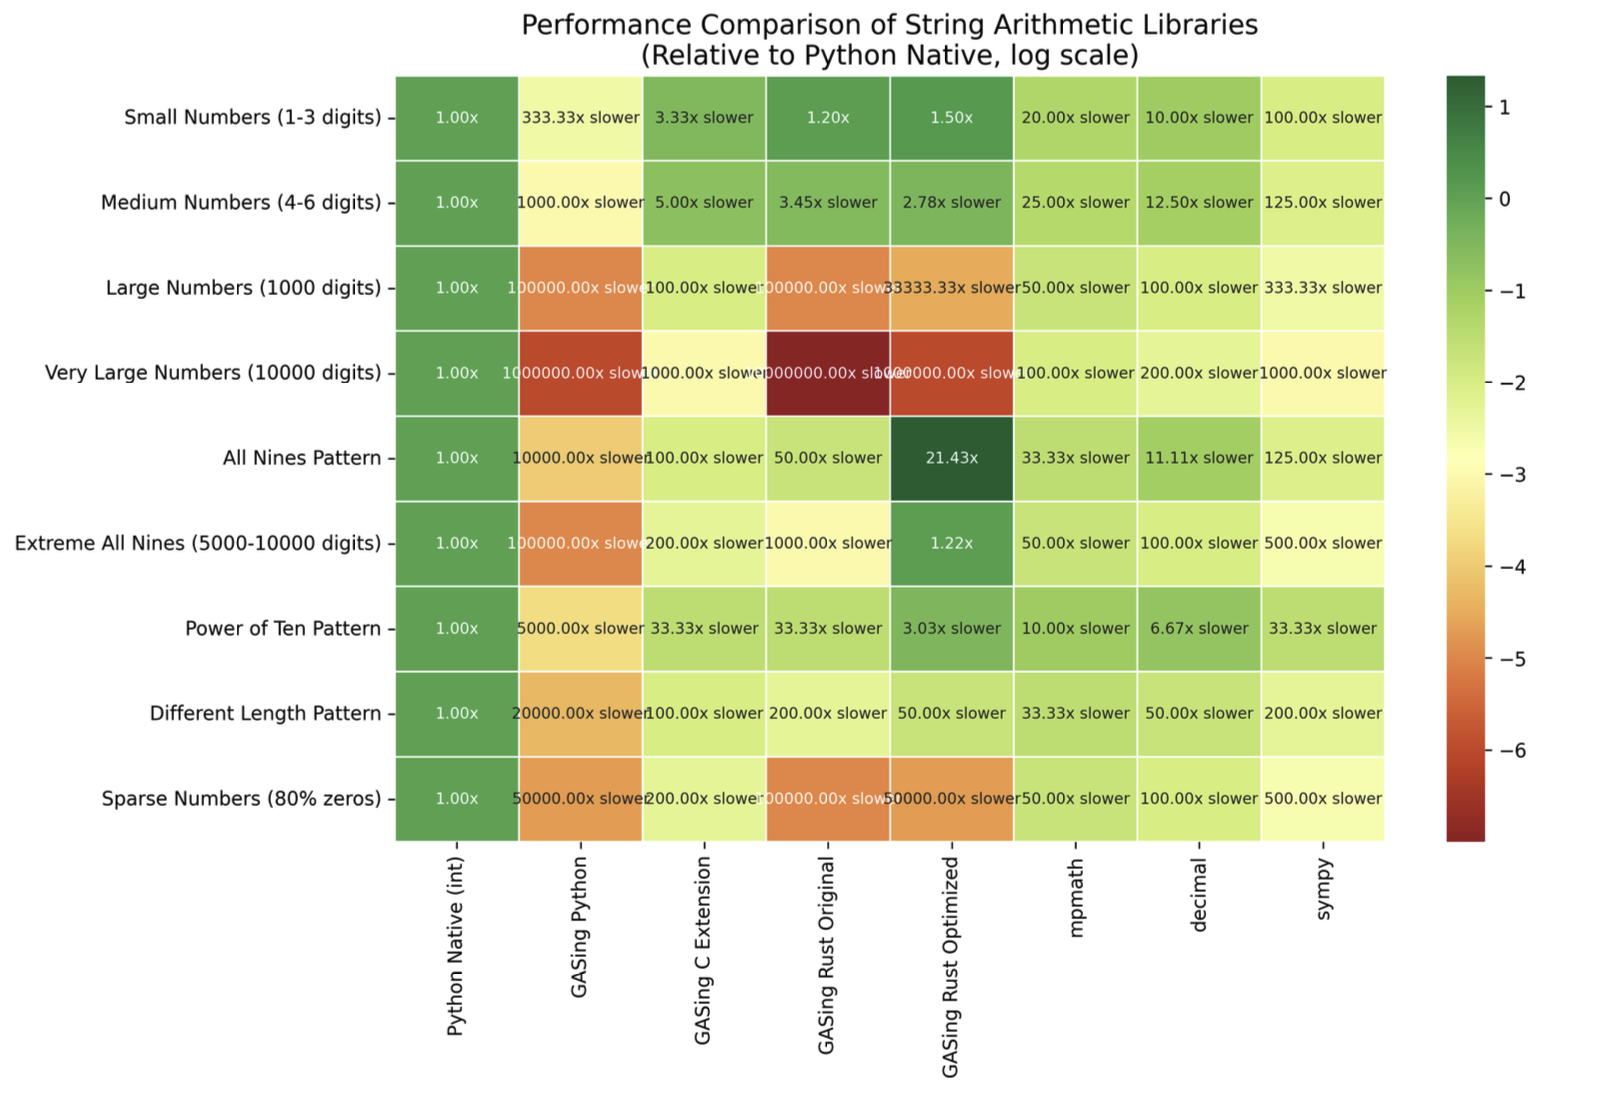
\includegraphics[width=\linewidth]{images/StringArithmetic.png}
  \caption{String Arithmetic}
  \label{fig:stringarithmetic}
\end{figure}



The following diagrams show the performance of different GASing implementations on the same set of algorithms applied to various number series for repeated applications of the same addition operations.

\begin{figure}[H]
  \centering
  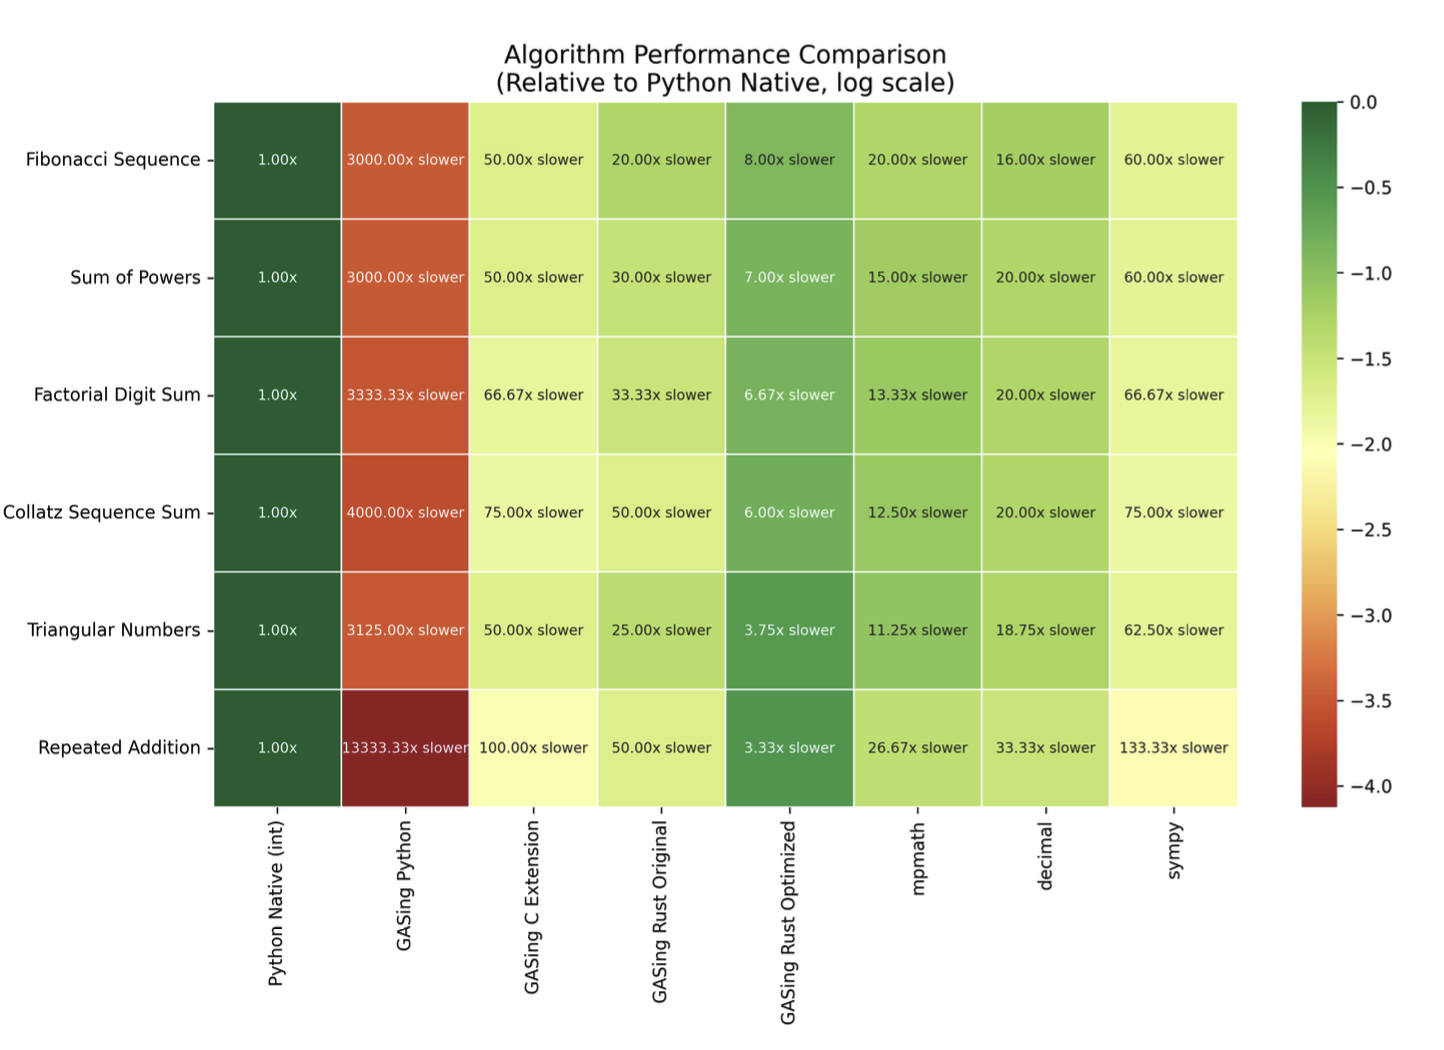
\includegraphics[width=\linewidth]{images/AlgorithmPerformanceComparison.png}
  \caption{Algorithmic Arithmetic}
  \label{fig:algorithmperformancecomparison}
\end{figure}



Looking ahead, these performance tests will be extended to arithmetic calculations that directly underpin large language model (LLM) inferencing. Since all inference operations in LLMs are ultimately arithmetic in nature—encompassing matrix multiplications, activations, and token transformations—any improvement in arithmetic efficiency translates directly to faster inference times and lower energy consumption at scale. This means that the resource savings demonstrated in these benchmarks could become highly visible and impactful in real-world AI deployments, especially as LLMs are deployed on increasingly resource-constrained or energy-sensitive platforms.

In summary, optimizing arithmetic operations through GASing principles has the potential to accelerate LLM inference, reduce operational costs, and make advanced AI systems more accessible and sustainable across a wide range of applications.


\section{Computational Advantages}
The GASing method offers several computational advantages that parallel key innovations in modern neural architectures, particularly those found in the Transformer model:
\paragraph{Locality of Reference and Token-Based Processing}

GASing's digit-wise processing conceptualizes numbers as sequences of tokens, similar to how Transformers process words or subwords. Just as the Transformer treats each token in a sentence as a discrete unit to be processed in parallel, GASing treats each digit as a computational token that can be addressed independently:

\begin{itemize}
\item \textbf{Tokenized Numerical Representation}: By treating a number as a sequence of digits, GASing effectively "tokenizes" numerical data. This mirrors how Transformers tokenize language, allowing arithmetic operations to be reframed as operations on token sequences rather than atomic values.
\end{itemize}

\begin{itemize}
\item \textbf{Cache-Friendly Operations}: The lookup-table approach enables high cache locality by organizing digit-wise operations into predictable memory access patterns. Similar to how Transformer's attention mechanism pre-computes key-value pairs, GASing pre-computes digit-wise results, reducing memory latency and improving throughput.
\end{itemize}

\begin{itemize}
\item \textbf{Compression at Representational Level}: This digit-wise representation provides a fundamental form of information compression. By recognizing patterns at the digit level (e.g., repeated digits, special sequences), GASing can compress computational workloads similar to how attention mechanisms compress sequence information through weighted summation.
\end{itemize}
\paragraph{Attention-Like Direct Accessibility and Predictable Branching}

GASing's systematic approach to arithmetic offers attention-like properties when processing multi-digit numbers:

\begin{itemize}
\item \textbf{Direct Digit Access}: Similar to how self-attention allows any position in a sequence to directly interact with any other position (O(1) path length), GASing's digit-wise processing enables direct access to any digit regardless of its position. This is especially powerful for operations that benefit from examining digits in specific positions.
\end{itemize}

\begin{itemize}
\item \textbf{Rule-Based Position Attention}: The systematic rule-based approach creates a form of "positional attention" where computational patterns are determined by digit positions and their relationships, much like how positional encodings in Transformers help the model understand sequence order.
\end{itemize}

\begin{itemize}
\item \textbf{Reduced Branch Mispredictions}: Like the deterministic attention mechanism in Transformers that avoids recurrent branching, GASing's predictable operation sequences reduce branch mispredictions in processor pipelines. This is particularly valuable in cases where traditional algorithms would have data-dependent branches.
\end{itemize}
\paragraph{Parallelization and Distributed Processing}

The digit-wise nature of GASing creates natural parallelization opportunities that mirror the Transformer's parallel processing capabilities:

\begin{itemize}
\item \textbf{Position-wise Processing}: Just as the Transformer applies the same feed-forward network to each position independently, GASing applies identical digit-wise operations across positions. This enables SIMD (Single Instruction, Multiple Data) optimization at the hardware level.
\end{itemize}

\begin{itemize}
\item \textbf{Granular Task Distribution}: GASing naturally decomposes arithmetic into smaller, independent sub-tasks that can be distributed across processing units, similar to how Transformer's multi-head attention parallelizes attention computations across multiple representation subspaces.
\end{itemize}

\begin{itemize}
\item \textbf{Constant Path Length Operations}: Like the Transformer's attention mechanism that maintains a constant computational path length regardless of sequence length, GASing's pattern-based approach provides constant-time operations for certain patterns regardless of digit count.
\end{itemize}
\paragraph{Information Compression and Pattern Recognition}

GASing represents a fundamental form of information compression that begins at the representational level:

\begin{itemize}
\item \textbf{Pattern-Specific Optimizations}: By identifying and exploiting digit patterns (repeating digits, special sequences), GASing achieves a form of numerical "semantic compression" analogous to how attention mechanisms learn to focus on relevant tokens while ignoring irrelevant ones.
\end{itemize}

\begin{itemize}
\item \textbf{Compositional Understanding}: GASing parses numbers as compositional entities with internal structure, much like how Transformers understand sentences as structured sequences. This allows arithmetic operations to leverage the compositional nature of numerical representation itself.
\end{itemize}

\begin{itemize}
\item \textbf{Adaptive Processing Depth}: For simple patterns, GASing can use shallow processing (direct lookup); for complex patterns, it can apply deeper, recursive processing—parallel to how Transformer layers process simple and complex linguistic patterns with varying attention distributions.
\end{itemize}


\section{Pedagogical Applications}
The GASing arithmetic method offers profound pedagogical advantages by making explicit the deep connections between elementary arithmetic and advanced mathematical concepts. By systematically reducing all operations to variations of addition while maintaining a digit-wise perspective, GASing provides students with a concrete pathway to understanding abstract algebraic structures and theoretical computer science principles.
\paragraph{Foundational Concepts Through Digit-Wise Operations}


\noindent\textbf{\textbf{Recursive Extensibility of Place Value}:} GASing's segment-wise processing demonstrates how the place value system is recursively extensible. Each digit position functions as a self-similar computational unit, mirroring the structure of formal languages and automata theory. This perspective helps students see arithmetic as a formal system with well-defined transformation rules.



\noindent\textbf{\textbf{From Concrete to Abstract Reasoning}:} The progression from single-digit addition to multi-digit operations and beyond illustrates how complex systems emerge from simple, well-defined rules—a fundamental concept in theoretical computer science. Students learn to recognize how higher-level abstractions are built from primitive operations.

\paragraph{Algebraic Structures in Elementary Arithmetic}

GASing's approach naturally leads students to discover abstract algebraic concepts through concrete numerical examples:


\noindent\textbf{\textbf{Monoidal Structure of Addition}:} The method's foundation on addition directly demonstrates the monoidal structure $(\mathbb{N}, +, 0)$, where:


\noindent The set of natural numbers is closed under addition


\noindent Addition is associative (crucial for parallel processing)


\noindent Zero serves as the identity element



\noindent\textbf{\textbf{Group-Theoretic Patterns}:} Through complement-based subtraction, students encounter their first examples of inverse operations, laying the groundwork for understanding group theory. The digit-wise approach makes these abstract concepts tangible by grounding them in familiar numerical operations.

\paragraph{Computational Thinking and Pattern Recognition}


\noindent\textbf{\textbf{Algorithmic Decomposition}:} GASing's step-by-step methodology teaches students to break down complex operations into simpler, manageable components—a core principle of computational thinking.



\noindent\textbf{\textbf{Pattern Recognition and Optimization}:} By working with digit patterns, students develop skills in identifying computational shortcuts and optimizations, directly applicable to algorithm design and analysis.



\noindent\textbf{\textbf{Finite State Automata}:} The carry propagation mechanism in multi-digit addition serves as an accessible introduction to finite state machines, with each digit position representing a state transition based on the current digit and incoming carry.

\paragraph{Pedagogical Advantages for Advanced Topics}


\noindent\textbf{\textbf{Topological Properties of Computation}:} The segment-wise processing in GASing illustrates how computational complexity can be managed through appropriate problem decomposition—a concept that scales to advanced topics in computational topology and distributed systems.



\noindent\textbf{\textbf{Category Theory Connections}:} The method's emphasis on compositionality and universal properties provides an intuitive entry point to category theory concepts, where addition serves as a prototypical example of a monoidal operation.



\noindent\textbf{\textbf{Type Systems and Formal Verification}:} GASing's explicit treatment of digit constraints and carry propagation introduces students to concepts of type safety and formal verification in a concrete, numerical context.

\paragraph{Cognitive Benefits and Practical Applications}


\noindent\textbf{\textbf{Reduced Cognitive Load}:} By focusing on a single core operation (addition) and systematically building complexity, GASing aligns with cognitive load theory, making advanced mathematical concepts more accessible.



\noindent\textbf{\textbf{Transferable Problem-Solving Skills}:} The pattern recognition and decomposition strategies learned through GASing transfer to programming, algorithm design, and other STEM disciplines.



\noindent\textbf{\textbf{Bridging Symbolic and Numerical Reasoning}:} The method's emphasis on the structural aspects of arithmetic helps students develop the ability to move fluidly between concrete computation and abstract reasoning.


Educational observations demonstrate that students who learn arithmetic through the GASing method develop not just computational fluency, but also a deeper appreciation for the underlying mathematical structures. This foundation enables them to approach advanced topics in computer science and mathematics with confidence, seeing the connections between elementary operations and complex theoretical constructs. The method's emphasis on a minimal, coherent operational vocabulary—grounded in addition but extending to higher mathematics—provides a powerful framework for developing both technical skills and conceptual understanding across the mathematical sciences.


\section{Future Directions and Discussion}
As artificial intelligence advances, the challenge of verifying and interpreting complex reasoning grows ever more critical. The Absolute Zero Reasoner (AZR) paradigm demonstrates that it is possible to achieve state-of-the-art reasoning capabilities without any human-curated data, relying solely on self-play and verifiable arithmetic operations as the grouding truth. This paradigm shift aligns directly with the GASing philosophy: arithmetic, especially addition and its extensions, provides a self-sufficient, axiomatically grounded framework for verifying the correctness of reasoning—independent of external supervision, hardware architecture, or computational paradigm.
\paragraph{The GASing Method as a Universal Computational Framework}

\textbf{By grounding AI-powered reasoning in well-documented, human-understandable conceptual abstractions like addition, we establish a truly universal computational framework with several critical properties:}

\begin{itemize}
\item \textbf{Platform-Agnostic:} The GASing framework remains equally valid and effective across all computing platforms:
\end{itemize}
  - Classical von Neumann architectures
  - Neuromorphic processors
  - Quantum computing systems (gate-based, annealing-based, or photonic)
  - Future computational paradigms not yet conceived

\begin{itemize}
\item \textbf{Algorithm-Agnostic:} Verification mechanisms depend solely on the mathematical properties of addition, not on specific algorithmic implementations:
\end{itemize}
  - Independent of programming language or software framework
  - Transcends differences between symbolic and neural approaches
  - Applicable to both deterministic and probabilistic methods
  - Maintains validity across domain-specific optimization techniques

\begin{itemize}
\item \textbf{Resource-Agnostic:} The framework provides a universal unit of resource measurement applicable across computational contexts:
\end{itemize}
  - Independent of specific hardware constraints (memory, processing units, energy)
  - Scalable from edge devices to supercomputers
  - Adaptable to varying precision requirements
  - Enables precise resource accounting in heterogeneous computing environments

\begin{itemize}
\item \textbf{Axiomatically Grounded:} Arithmetic serves as a definitive framework that establishes clear boundaries of rational precision:
\end{itemize}
  - Provides a formal basis for all computational correctness claims
  - Establishes unambiguous termination conditions for decision processes
  - Enables verification chains with guaranteed consistency
  - Creates a universal standard for precision and approximation

The correctness verification mechanisms can always be traced back to the axiomatic definition of addition and the finite vocabulary admitted in each application context. While this vocabulary adapts to different domains, it remains terminable in decision processes because it builds on fundamental arithmetic operations with clear termination conditions, regardless of the physical substrate performing the calculation.
\paragraph{Arithmetic as the Universal Computational Substrate}

It is crucial to recognize that all computations—regardless of their apparent complexity or implementation—reduce to arithmetic operations at their logical foundation:

\begin{itemize}
\item \textbf{Universal Computational Mapping:}
\end{itemize}
  - Every token prediction in language models → Matrix operations → Addition sequences
  - Quantum gate operations → Unitary transformations → Complex number arithmetic
  - Neural network activations → Weighted sums and non-linear functions → Addition and multiplication
  - Symbolic reasoning → Logical operations → Arithmetic on truth values

\begin{itemize}
\item \textbf{Hardware-Independent Optimization:}
\end{itemize}
  - Pre-computation of recurring patterns yields benefits regardless of physical implementation
  - Pattern recognition strategies remain valid across all computing architectures
  - Resource optimization techniques are transferable between computational paradigms
  - Lookup mechanisms provide acceleration whether implemented in classical or quantum systems

Similar to the arguments presented in AZR's framework for abduction, deduction, and induction is not merely a high-level abstraction; each of these reasoning modes is ultimately reducible to arithmetic operations, most notably matrix dot products. These operations serve as the computational substrate for verifying hypotheses, generating explanations, and drawing inferences. By grounding all reasoning in arithmetic, GASing together offer a path toward:

1. \textbf{Self-Sufficient Verification of Truth}: Arithmetic rules, being universally accepted and axiomatically defined, enable models to autonomously verify the correctness of their outputs. This eliminates the need for human-provided labels or curated datasets, allowing for open-ended, scalable learning and reasoning.

2. \textbf{Unified Framework for Reasoning}: Abduction (hypothesis generation), deduction (logical consequence), and induction (pattern discovery) can all be formalized as arithmetic operations—often as matrix multiplications or dot products—within the AZR paradigm. This unification simplifies the architecture of reasoning systems and ensures that all forms of inference are ultimately transparent and verifiable.

3. \textbf{Enhanced AI Interpretability and Trust}: By reducing complex reasoning to sequences of arithmetic steps, the entire process becomes auditable and explainable. Each step can be traced back to fundamental operations, making it possible to verify not just the final answer but the entire chain of reasoning.

4. \textbf{Bridging Symbolic and Sub-symbolic AI}: The arithmetic foundation enables seamless integration between symbolic logic (rules, proofs) and sub-symbolic computation (matrix operations, neural activations). This hybrid approach supports both human-understandable explanations and efficient machine computation.

5. \textbf{Preparation for Autonomous, Superhuman AI}: As demonstrated by AZR, models can propose, solve, and verify tasks entirely through self-play, guided by arithmetic truth. This prepares AI systems for a future where they must operate and improve independently, without relying on human supervision or external data.

As detailed in recent work on the Absolute Zero Reasoner (AZR), the three primary modes of learning—deduction, abduction, and induction—can be mapped directly onto the fundamental arithmetic operations of subtraction, addition, and multiplication/division, respectively. Deduction resembles subtraction, isolating unknowns from knowns; abduction parallels addition, combining elements to reach a target; and induction aligns with multiplication/division, generalizing or partitioning patterns. This mapping is not merely metaphorical: AZR operationalizes each reasoning mode as arithmetic, typically via matrix dot products and related operations. Thus, the logical and functional structure of arithmetic is sufficiently expressive to serve as the substrate for all forms of inference, unifying symbolic and sub-symbolic reasoning.

Anthropic's groundbreaking work on monosemanticity ("Towards Monosemanticity: Decomposing Language Models With Dictionary Learning") provides compelling evidence for this approach. Their research demonstrated that sparse autoencoders can decompose complex language models into thousands of interpretable features, with each feature representing a specific, meaningful pattern—similar to how GASing decomposes complex arithmetic into modular, pattern-recognizing steps. They discovered that just 512 neurons can effectively represent tens of thousands of features, and these features connect in "finite-state automata"-like systems to implement complex behaviors.

This directly parallels GASing's principle of pattern decomposition: where Anthropic finds that complex language behaviors can be decomposed into interpretable components, GASing shows that complex arithmetic can be decomposed into pattern-driven addition operations. Both approaches tackle the "curse of dimensionality" by identifying compositional building blocks that make complex systems interpretable and controllable.

Furthermore, Anthropic demonstrated that these monosemantic features can be used to intervene on and steer transformer generation—activating a specific feature (like "base64" or "Arabic script") causes the model to generate text with those characteristics. In the GASing framework, recognizing specific numerical patterns similarly allows for targeted optimizations and controlled behaviors.

The key insight connecting these approaches is that dictionaries and lookup tables are essentially pre-computed results—cached knowledge that can dramatically accelerate reasoning when leveraged appropriately. This parallel between GASing and Anthropic's approach reveals a profound connection between mental arithmetic and neural computation.
\paragraph{Monosemanticity and Digit-Wise Decomposition}

Anthropic's dictionary learning approach in their Monosemantic research represents a breakthrough in neural network interpretability through decomposition. Their technique addresses the "polysemanticity problem" where individual neurons encode multiple concepts simultaneously, making interpretation difficult. Using sparse autoencoders, they decompose these mixed neural activations into thousands of interpretable "features" or "basis vectors" that represent singular concepts—such as specific text patterns, data formats, or linguistic structures.

This decomposition is structurally analogous to how GASing decomposes complex arithmetic operations into digit-wise patterns:

- \textbf{GASing's Lookup Tables}: Break down arithmetic operations into pre-computed digit-wise patterns stored in mental lookup tables
- \textbf{Anthropic's Dictionary Elements}: Break down neural activations into interpretable monosemantic features stored in sparse feature vectors

In both cases, complex operations (whether arithmetic calculations or neural processes) are transformed into combinations of simpler, more interpretable components that can be efficiently accessed and combined.
\paragraph{From Polynomial Types to Computational Efficiency}

This dictionary-based filtering methodology bears remarkable structural similarity to \textbf{[[Polynomial Functors]]} as in [[Category Theory]], where arithmetic rules denote different types of information and their compositional relationships. Just as Polynomial Functors use addition to represent alternatives and multiplication to represent combinations, both GASing's lookup patterns and Anthropic's dictionary features create formal algebras for organizing computational resources:

- In GASing: Digit patterns become the "vocabulary" of arithmetic, with rules for composition that minimize cognitive effort
- In Anthropic's approach: Dictionary features become the "vocabulary" of neural computation, with sparse activations that minimize computational resources

The dictionary learning approach is fundamentally a form of resource-aware computation that aligns directly with [[Linear Logic]] principles—each feature is consumed exactly once in reconstructing the neural activation, just as each digit pattern is consumed exactly once in GASing's mental calculations.
\paragraph{Practical Implications for Computation}

The digit-wise pattern extraction strategy in GASing arithmetic represents a fundamental breakthrough in computational efficiency, with deep connections to advanced mathematical frameworks like [[Homological Algebra]] and [[Topological Data Analysis]] (TDA). These fields, at the forefront of modern data science, employ similar pattern recognition and dimensional reduction techniques to extract meaningful structure from complex datasets.

The algebraic topology underpinning these approaches—particularly the computation of persistent homology in TDA—shares striking parallels with GASing's digit-wise operations. Both frameworks excel at identifying and exploiting qualitative features that persist across multiple scales, enabling more efficient representation and manipulation of complex data structures. This connection to [[Persistent Homology]] and [[Morse Theory]] provides a rigorous mathematical foundation for understanding how GASing's pattern-based approach achieves its remarkable computational efficiency.

Just as GASing enables humans to perform complex mental calculations through pattern recognition and recombination, modern neural architectures leverage similar principles rooted in [[Sheaf Theory]] and [[Category Theory]]. In Anthropic's experiments with Claude 3 Sonnet, the decomposition of neural layers into interpretable features mirrors the way [[Čech Complexes]] in TDA capture topological features across different scales. This multi-scale pattern recognition allows systems to:

1. \textbf{Dynamically renormalize} computational processes using techniques inspired by [[Renormalization Groups]] in theoretical physics
2. \textbf{Cache and reuse} intermediate results through structures analogous to [[Cohomology Operations]] in algebraic topology
3. \textbf{Adaptively allocate resources} using methods that parallel [[Barcodes]] in persistent homology, which track the persistence of topological features across scales

The mathematical framework of [[Spectral Sequences]] from homological algebra provides a powerful lens for understanding how GASing's digit-wise operations can efficiently navigate complex computational landscapes. This connection to advanced algebraic topology explains why GASing's approach remains effective even as computational paradigms evolve—the underlying mathematical structures are fundamentally stable across different representations and implementations.

The real challenge, for both humans and machines, is to access these pre-computed patterns with minimal resource expenditure while adapting retrieval strategies to the local context. The GASing framework's modular, segment-wise approach provides a principled foundation for this adaptive resource management, with deep connections to [[Sheaf Cohomology]] and its applications in distributed systems and data analysis.

By establishing addition as the foundational operator for all reasoning mechanisms, GASing provides an abstract, universal unit of resource measurement that finds elegant expression in the language of [[Category Theory]] and [[Homotopy Type Theory]]. This approach enables precise assessment of computational requirements through the lens of [[Euler's Characteristic]] and other topological invariants, creating a rigorous framework for reasoning about computational complexity across different scales and representations.

\textbf{The profound advantage of this approach is that it provides a mathematical foundation for understanding how complex computations can be decomposed into simpler, more manageable components—a principle that lies at the heart of both GASing arithmetic and modern topological methods in data science.} This separation creates an enduring bridge between theoretical verification and practical optimization across all computational paradigms. Even as we transition through classical computing to neuromorphic systems and ultimately to mature quantum computing, the core verification mechanisms remain mathematically identical because they depend only on the abstract properties of addition and topological invariants, not on the physical substrate performing the operations.

More importantly, this mathematical framing enables us to view each LLM as a custom numerical system with its own unique arithmetic properties, where the token distributions, weight matrices, and activation patterns constitute a rich numerical ecosystem. The principles of [[Representation Stability]] from [[homological algebra]] suggest that many of the patterns we discover in these systems will remain stable even as the underlying models scale, providing a powerful tool for model compression and optimization. By identifying and exploiting these stable patterns—much like how TDA identifies persistent topological features—we can achieve significant computational savings while preserving model accuracy and interpretability.

These insights are not merely theoretical: they provide immediately actionable approaches for optimizing existing AI systems while pointing the way toward more efficient and interpretable architectures. The deep mathematical connections between GASing arithmetic, homological algebra, and topological data analysis suggest that we are only beginning to understand the full potential of these approaches for building the next generation of intelligent systems.


\section{Conclusion}
\paragraph{Cultural and Historical Context: Ethno Arithmetic and Fractal Patterns}

The GASing method finds profound resonance with the work of Professor Ron Eglash on \textbf{Ethno Arithmetic} and fractal patterns in Indigenous knowledge systems. Eglash's research (Eglash, 1999) demonstrates how many African, Native American, and other Indigenous cultures developed sophisticated mathematical concepts through fractal patterns in their art, architecture, and social organizations. These patterns, often embedded in cultural practices, represent an early form of \textbf{progressive function application} and \textbf{self-similar computation} that predates Western formal mathematics.

GASing's digit-wise, cell-like modules parallel the recursive, self-similar structures found in Indigenous fractal designs, where complex patterns emerge from the repeated application of simple rules—a principle that mirrors GASing's approach to arithmetic through the progressive application of addition. The \textbf{combinatorial patterns} in GASing's digit-wise processing echo the recursive geometric transformations observed in African fractals, where simple scaling rules generate complex, computationally rich structures.

This connection is particularly significant because it suggests that GASing's approach is not merely a technical innovation but part of a broader human tradition of pattern-based computation. By recognizing these parallels, GASing bridges modern computational thinking with historical mathematical practices, creating a more inclusive framework that honors diverse mathematical traditions while providing a foundation for future computational paradigms.
\paragraph{Computational Foundations}

The GASing arithmetic method positions the foundational architecture of computing tasks by elevating addition to the role of meta-operator—a universal primitive from which all arithmetic logic operations can be systematically constructed, analyzed, and verified. This reductionist approach is not merely a theoretical exercise; it provides a practical, measurable framework for assessing resource consumption, numerical precision, and logical correctness in both human and machine reasoning. As modern LLM technologies have conclusively demonstrated, even \textbf{the most sophisticated reasoning and content generation processes}—from poetry composition to mathematical proof generation—\textbf{can be carried out with arithmetic operations} as their fundamental computational substrate. The seemingly magical capabilities of these systems emerge entirely from operations that, at their core, are nothing more than carefully orchestrated \textbf{patterns of addition and multiplication}.

By \textbf{conceptually decomposing} complex operations such as multiplication, subtraction, and division into sequences of segment-wise additions, GASing enables explicit quantification of computational effort: every operation is traceable to a countable set of addition-equivalent steps. This transparency allows for rigorous evaluation and optimization of both cognitive and computational resource usage, offering a clear metric for comparing algorithms, implementations, or even reasoning strategies. Such granularity is invaluable for designing systems—human or artificial—that must operate within strict resource constraints, whether those are working memory, processing time, or energy consumption.

GASing’s focus on addition as the core operator also underpins a unified, cross-referential decision framework. By expressing all arithmetic logic in terms of addition, the method ensures that every step is both interpretable and verifiable, supporting robust provenance tracking and error detection. This unification bridges symbolic and sub-symbolic computation, aligning the clarity of rule-based logic with the efficiency of neural and matrix-based operations. The result is a system where numerical precision and logical correctness are not competing priorities, but mutually reinforcing outcomes of a single, transparent process.

Originally conceived to accelerate arithmetic calculation and reduce cognitive load for learners, GASing’s segment-wise, pattern-driven approach is grounded in well-established cognitive principles, such as chunking and resource preservation. It empowers users to adapt the granularity of operations to their own cognitive limits, minimizing mental effort while maximizing accuracy and speed. This adaptability is mirrored in modern AI, where resource management and interpretability are critical for scaling intelligent systems.

In summary, GASing arithmetic is more than a pedagogical innovation—it is a rigorous, interpretable, and scalable substrate for reasoning that bridges the gap between human cognition and machine computation. By grounding all operations in addition, GASing delivers a framework where every logical step is measurable, every result is verifiable, and every computation is optimized for resource efficiency.

At a deeper level, GASing establishes \textbf{\textbf{\textit{addition}}} as a universal atomic "token" of computational effort—a fundamental unit of measure that enables precise resource accounting across all computational contexts, from silicon chips to human minds. This resource-aware arithmetic framework redefines how we attribute and measure cognitive and computational work, creating a unified currency of effort that makes the cost of any reasoning process explicitly quantifiable. Each "adding action" becomes a credit unit within a universal ledger of computational activity, allowing systems to track, allocate, and optimize resources with unprecedented granularity. This approach transcends traditional hardware-specific metrics (like CPU cycles or memory usage) to establish a hardware-agnostic measure of fundamental reasoning operations.

This philosophical reinterpretation of what counting fundamentally means represents a major advancement in how we conceptualize and accumulate knowledge about the world. By establishing the addition operation as the atomic unit of reasoning, GASing provides a common denominator for measuring all forms of information processing, creating a bridge between disparate computational paradigms—quantum, neural, symbolic—and human cognition. It enables precise verification chains that can track not just the results of computation, but the exact resource cost of arriving at those results, providing a meta-level framework for reasoning about reasoning itself.

Intellectually, grounding all computational tasks in a single unifying operator yields an additional, profound benefit: it encourages both human and machine minds to converge on a shared pattern of reasoning. This shared pattern not only accumulates experience and impressions, but also aligns prior intentions and fosters deeper mutual understanding. In the abstract, aligning minds—whether individual, collective, or artificial—around a common operator is a necessary condition for establishing a unified theory of learning. Only by sharing such a foundational operator can human, machine, or organizational learning truly converge on a common framework, enabling the transfer and accumulation of knowledge, experience, and intention across all forms of intelligence.

As AI systems become increasingly autonomous and integrated into human workflows, such foundational clarity and measurability will be essential for ensuring trust, transparency, and continual improvement in both artificial and human intelligence. Modern LLMs have definitively proven that even the most advanced cognitive-seeming tasks—from multimodal reasoning to creative problem-solving—ultimately resolve to sequences of arithmetic operations. This revelation means that optimizing these fundamental operations is not merely an engineering detail but a strategic imperative with cascading benefits for AI capabilities, energy consumption, and accessibility. By \textbf{minimizing the resource footprint of these basic arithmetic operations through the principles outlined in GASing}, we can achieve dramatic improvements in these proven useful and pragmatic AI applications regardless of their apparent complexity or sophistication.

\textbf{Crucially, by grounding AI-powered reasoning in well-documented and human-understandable conceptual abstractions, GASing eliminates dependencies on specific hardware or software implementations.} The correctness verification process can always be traced back to the axiomatic definition of addition and the finite vocabulary admitted in each application context. This creates an adaptive yet fundamentally terminable reasoning framework—one that can evolve with technological advances without losing its verifiability. As hardware implementations evolve from classical computing to neuromorphic processors or quantum computers, the GASing verification mechanisms remain stable and interpretable to humans because they depend on mathematical properties, not implementation details. This ensures a consistent standard of correctness while enabling continuous innovation in the underlying technologies.

GASing's commitment to a minimal, interpretable operational vocabulary thus stands as both a practical solution and a philosophical imperative for the future of collaborative reasoning—one where the economics of knowledge acquisition can be precisely quantified, compared, and optimized across the full spectrum of computational agents, from the simplest calculator to the most sophisticated AI system to the human mind itself.

% Appendix section
\appendix
% Appendix
% This appendix contains supplementary material, proofs, extended algorithms, and additional data relevant to the GASing Arithmetic System.

\section{Appendix I: GASing Addition Algorithm}
\label{appendix:addition}
\begin{lstlisting}[language=Python,caption={GASing Addition Algorithm}]
function GASing_Addition(a, b):
    result = ""
    carry = 0
    
    # Pad the shorter number with leading zeros
    a = pad_with_zeros(a, len(b))
    b = pad_with_zeros(b, len(a))
    
    # Process from left to right
    for i in range(0, len(a)):
        # Add digits and carry
        digit_sum = int(a[i]) + int(b[i]) + carry
        
        # Determine new digit and carry
        if digit_sum > 9:
            carry = 1
            digit = digit_sum - 10
        else:
            carry = 0
            digit = digit_sum
        
        result += str(digit)
    
    # Add final carry if necessary
    if carry > 0:
        result += str(carry)
        
    return result
\end{lstlisting}

\section{Appendix II: GASing Multiplication Algorithm}
\label{appendix:multiplication}
\begin{lstlisting}[language=Python,caption={GASing Multiplication Algorithm (Conceptual)}]
function GASing_Multiplication(a, b):
    # Initialize a grid to store partial products (results of single-digit multiplications)
    # The dimensions of the grid depend on the number of digits/segments in a and b.
    # For example, if a has M segments and b has N segments, grid is N x M.
        
    grid = initialize_partial_product_grid(a, b) # Each grid[i][j] = segment_b[i] * segment_a[j]
        
    # The core of multiplication is now to sum the values in this grid in a structured way.
    # This can be visualized as summing diagonals or columns, applying GASing addition.
    # For simplicity, imagine a function that collects these partial products and sums them
    # using the previously defined GASing_Addition logic, managing carries appropriately.

    final_product = "0"
    # Iterate through the grid, treating each row (or shifted row) as a number to be added.
    # This is a conceptual representation; actual implementation involves careful alignment and summation.
    for i in range(len(b)):
        partial_sum_for_row_i = "0"
        for j in range(len(a)):
            # Conceptually, each grid[i][j] contributes to a sum that is then added.
            # A more direct approach involves summing diagonals or columns with carries.
            # This step is a placeholder for the detailed grid summation logic.
            # For instance, grid[i][j] is like (digit_b[i] * digit_a[j]) * 10^(position_factor)
            # These terms are then summed up.
            pass # Detailed grid summation logic would be here.

    # A more accurate representation of grid summation:
    # 1. Calculate all single-segment products: product_ij = segment_a[j] * segment_b[i]
    # 2. Arrange these products in a grid, aligning them according to their place value.
    # 3. Sum the columns of this grid using GASing_Addition, propagating carries.

    # Example (conceptual): Summing diagonals of the grid of partial products
    # result = sum_grid_diagonals_with_gasing_addition(grid)

    # Simplified placeholder for the complex summation logic:
    # Assume 'grid_to_result' performs the systematic addition of partial products
    # according to GASing principles (left-to-right, carry management).
    
    result = perform_structured_addition_on_grid(grid, GASing_Addition_function_pointer)

return result
\end{lstlisting}

\section{Appendix III: GASing Subtraction and Division Algorithms}
\label{appendix:subtraction}
\begin{lstlisting}[language=Python,caption={GASing Subtraction Algorithm}]
function GASing_Subtraction(a, b, base=10):
    # Ensure a and b are of the same length for complement calculation
    # This might involve padding the shorter number or defining a fixed width.
    # For simplicity, assume a and b are positive integers represented as strings.
    num_digits = max(len(a), len(b))

    a_padded = pad_with_zeros(a, num_digits)
    b_padded = pad_with_zeros(b, num_digits)

    # Calculate n's complement of b (e.g., ten's complement for base 10)
    # This involves (base^num_digits - b_padded)
    # A common method: ( (base-1)'s_complement of b_padded ) + 1
    b_complement_n_minus_1 = ""
    for digit_char in b_padded:
        b_complement_n_minus_1 += str((base - 1) - int(digit_char))

    # Add 1 to get n's complement (e.g., ten's complement)
    # This addition itself can use a simplified version of GASing_Addition or direct logic
    one_str = pad_with_zeros("1", num_digits)
    b_complement_n = GASing_Addition(b_complement_n_minus_1, one_str) # Assuming base compatibility
    # Handle potential overflow from complement addition if b_complement_n exceeds num_digits
    if len(b_complement_n) > num_digits and b_complement_n.startswith('1'): # Check for leading '1' from carry
        b_complement_n = b_complement_n[1:] # Keep only num_digits
    else:
        b_complement_n = pad_with_zeros(b_complement_n, num_digits)

    # Perform a + (n's complement of b)
    # The GASing_Addition function is used here.
    sum_with_complement = GASing_Addition(a_padded, b_complement_n) # Ensure base compatibility

    # Interpret the result
    if len(sum_with_complement) > num_digits and sum_with_complement.startswith('1'): # Overflow carry indicates positive result
        result = sum_with_complement[1:] # Discard overflow carry
        is_negative = False
    else:
        # No overflow carry indicates negative result or zero
        # The result is negative, and its magnitude is the n's complement of sum_with_complement
        # For simplicity, we'll just flag it as negative and take complement again for magnitude
        # (or handle based on specific complement arithmetic rules)
        if sum_with_complement == pad_with_zeros("0", num_digits):
            result = sum_with_complement
            is_negative = False
        else:
            # Recalculate n's complement of sum_with_complement to get magnitude
            temp_complement_n_minus_1 = ""
            sum_with_complement_padded = pad_with_zeros(sum_with_complement, num_digits)
            for digit_char in sum_with_complement_padded:
                temp_complement_n_minus_1 += str((base - 1) - int(digit_char))
            result = GASing_Addition(temp_complement_n_minus_1, one_str) # Magnitude
            if len(result) > num_digits and result.startswith('1'):
                result = result[1:]
            else:
                result = pad_with_zeros(result, num_digits)
            is_negative = True
            
    return result, is_negative
\end{lstlisting}

\begin{lstlisting}[language=Python,caption={GASing Division Algorithm}]
function GASing_Division(dividend, divisor, base=10):
    if divisor == pad_with_zeros("0", len(divisor)):
        return "Error: Division by zero"
    quotient = "0"
    current_dividend = dividend
    one = pad_with_zeros("1", len(quotient)) # For incrementing quotient

    # Repeatedly subtract divisor from current_dividend
    # We need a comparison function: is_greater_or_equal(num1, num2)
    while is_greater_or_equal(current_dividend, divisor):
        subtraction_result, is_neg = GASing_Subtraction(current_dividend, divisor, base)
        if is_neg: # Should not happen if is_greater_or_equal is correct
            break 
        current_dividend = subtraction_result
        quotient = GASing_Addition(quotient, one) # Increment quotient
        # Ensure 'one' is padded correctly if quotient grows
        if len(quotient) > len(one):
            one = pad_with_zeros("1", len(quotient))
        elif len(one) > len(quotient):
            quotient = pad_with_zeros(quotient, len(one))

    remainder = current_dividend
    return quotient, remainder
\end{lstlisting}




% Old section inclusions are commented out for reference
% \sectionheader{Background and Related Work}
\label{sec:background}

\subsection{Petri Net Fundamentals}

Formally, a Petri Net is a tuple $(P, T, F, M_0)$ where:
\begin{itemize}
    \item $P$ is a finite set of places
    \item $T$ is a finite set of transitions
    \item $F \subseteq (P \times T) \cup (T \times P)$ is a set of arcs
    \item $M_0: P \rightarrow \mathbb{N}$ is the initial marking
\end{itemize}

The dynamics of Petri Nets are governed by the firing of transitions. A transition $t$ is enabled if each input place $p$ has at least as many tokens as the weight of the arc from $p$ to $t$. When a transition fires, it consumes tokens from its input places and produces tokens in its output places according to the weights of the corresponding arcs.

\subsection{Types of Petri Nets}

Several extensions to the basic Petri Net model have been proposed to enhance its modeling power:

\begin{itemize}
    \item \textbf{Colored Petri Nets} \cite{jensen1987coloured}: Extend the basic model by allowing tokens to have data values (colors).
    \item \textbf{Timed Petri Nets}: Incorporate time into the model, allowing for the analysis of temporal properties.
    \item \textbf{Stochastic Petri Nets}: Introduce probabilistic elements to model random behavior.
    \item \textbf{Hierarchical Petri Nets}: Allow for the decomposition of complex models into simpler submodels.
\end{itemize}

\subsection{Applications of Petri Nets}

Petri Nets have been applied to various domains, including:

\begin{itemize}
    \item \textbf{Workflow Management} \cite{van2000workflow}: Modeling and analyzing business processes.
    \item \textbf{Manufacturing Systems}: Modeling production lines and resource allocation.
    \item \textbf{Communication Protocols}: Analyzing the behavior of network protocols.
    \item \textbf{Software Design}: Modeling concurrent and distributed software systems.
\end{itemize}

\subsection{Related Work}

Petri Nets have been extended in various ways to model complex systems, but their integration with tensor algebra is relatively unexplored. Tensors provide a natural language for encoding multidimensional relationships and parallel computations, making them ideal for representing the state and evolution of Petri Nets with topological structure.

David Spivak’s work on polynomial functors provides a categorical framework for modeling data types and processes as compositional, tree-like structures. This perspective aligns naturally with Petri Nets, where transitions can be seen as functorial operations on collections of tokens, and places as objects in a category.

Digit-wise arithmetic is a canonical example of a computation that is both highly structured and parallelizable. Neural-symbolic systems have struggled to capture such computations in a transparent and generalizable way. By modeling digit-wise arithmetic as a tensorized Petri Net, we can make explicit the flow of information and the compositional structure of the computation.
% \sectionheader{Methodology}
\label{sec:methodology}

\subsection{Tensorized Petri Nets via Polynomial Functors}

\subsubsection{Tensor Representation of Petri Nets}

\begin{itemize}
    \item \textbf{Places as Tensor Indices:} Each place in a Petri Net corresponds to an index in a tensor, representing a position (e.g., a digit in a number, or a cell in a grid).
    \item \textbf{Tokens as Tensor Entries:} The state of the net is encoded as a tensor, with entries indicating the presence or value of tokens at each place.
    \item \textbf{Transitions as Tensor Operations:} Transitions correspond to multilinear maps or contractions, updating the tensor state according to the net’s rules.
\end{itemize}

\subsubsection{Polynomial Functors for Compositionality}

\begin{itemize}
    \item \textbf{Elements as Operators and Operands:} Inspired by polynomial functors, each element (place or transition) can act as both an operand (receiving tokens) and an operator (transforming tokens).
    \item \textbf{Functorial Structure:} The wiring of the Petri Net encodes a functorial mapping from input tensors (operands) to output tensors (results), supporting modular and hierarchical composition.
\end{itemize}

\subsubsection{Example: Digit-wise Arithmetic}

\begin{itemize}
    \item \textbf{Digit Positions as Places:} Each digit position in a number is a place in the Petri Net.
    \item \textbf{Carry and Sum as Transitions:} Transitions implement digit-wise addition, carry propagation, and modular reduction, all as tensor operations.
    \item \textbf{Topological Relationships:} The tensor structure captures the adjacency of digits and the flow of carries, enabling parallel and interpretable computation.
\end{itemize}

\subsection{Problem Definition}

[Define the specific problem you are addressing with your Petri Net model]

\subsection{Proposed Petri Net Model}

Our proposed Petri Net model for [specific system or process] consists of the following components:

\begin{itemize}
    \item \textbf{Places}: Represent [specific states or conditions in your system]
    \item \textbf{Transitions}: Represent [specific events or actions in your system]
    \item \textbf{Tokens}: Represent [specific resources or entities in your system]
\end{itemize}

\begin{figure}[htbp]
\centering
\begin{tikzpicture}[node distance=1.5cm and 2.5cm, >=stealth, bend angle=45, auto] % Adjusted default node distances

% Define places with new coordinates for better layout
\placewithtokens{p1}{0,0}{2}        % Resource
\placewithtokens{p2}{5,0}{0}        % Process
\placewithtokens{p3}{2.5,-2.5}{1}    % Control
\placewithtokens{p4}{7.5,-2.5}{0}    % Output
\placewithtokens{p5}{2.5,-5.5}{0}    % Complete

% Define transitions with new coordinates
\node[transition] (t1) at (2.5,0) {};   % Start (between P1 and P2, above P3)
\node[transition] (t2) at (5,-2.5) {};  % Execute (between P2 and P4, aligned with P3)
\node[transition] (t3) at (1,-4) {};    % Cancel (below and to the left of P3, leading to P5)
\node[transition] (t4) at (4,-4) {};    % Finish (below and to the right of P3, or below T2, leading to P5)

% Define arcs (connections remain logically the same)
\draw[pre] (p1) -- (t1);
\draw[post] (t1) -- (p2);
\draw[pre] (p3) -- (t1);    % P3 is an input to T1
\draw[post] (t1) -- (p3);   % T1 returns a token to P3 (maintains control token)

\draw[pre] (p2) -- (t2);
\draw[pre] (p3) -- (t2);    % P3 is also an input to T2
\draw[post] (t2) -- (p4);

\draw[pre] (p3) -- (t3);
\draw[post] (t3) -- (p5);

\draw[pre] (p4) -- (t4);
\draw[post] (t4) -- (p5);

% Add labels (node anchors ensure they are placed relative to the node)
\node[above] at (p1.north) {Resource};
\node[above] at (p2.north) {Process};
\node[left] at (p3.west) {Control}; % Adjusted to left to avoid overlap with T1-P3 arc
\node[above] at (p4.north) {Output}; % Adjusted to above for consistency
\node[below] at (p5.south) {Complete};

\node[above] at (t1.north) {Start};
\node[above] at (t2.north) {Execute}; % Adjusted to above
\node[left] at (t3.west) {Cancel};
\node[right] at (t4.east) {Finish};

% Add a title
\node[above=1cm of p1.north -| t1.north] {Petri Net Model of a Simple Workflow Process}; % Position title relative to top elements

\end{tikzpicture}
\caption{Generic Petri Net model structure for [specific system or process]}
\label{fig:petri_net_generic_model}
\end{figure}

To illustrate common concurrency problems that can be modeled with Petri Nets, we present the Dining Philosophers problem (Figure \ref{fig:dining_philosophers}) and the Producer-Consumer problem (Figure \ref{fig:producer_consumer_workflow}).

\begin{figure*}[htbp]
\centering
% Petri Net Model of the Dining Philosophers Problem (Refined)
\begin{tikzpicture}[node distance=2.2cm and 2.2cm, >=stealth, bend angle=30, auto, on grid]
    % Philosopher thinking states
    \placewithtokens{p1}{0,0}{1}
    \placewithtokens{p2}{3,0}{1}
    \placewithtokens{p3}{1.5,-2.6}{1}

    % Philosopher eating states
    \placewithtokens{e1}{-1.2,-1.5}{0}
    \placewithtokens{e2}{4.2,-1.5}{0}
    \placewithtokens{e3}{1.5,-4.1}{0}

    % Forks
    \placewithtokens{f1}{0,-1.5}{1}
    \placewithtokens{f2}{3,-1.5}{1}
    \placewithtokens{f3}{1.5,-1.5}{1}

    % Transitions (pick up forks)
    \node[transition, rounded corners=2pt] (t1) [below left=0.7cm and 0.7cm of p1] {};
    \node[transition, rounded corners=2pt] (t2) [below right=0.7cm and 0.7cm of p2] {};
    \node[transition, rounded corners=2pt] (t3) [below=0.7cm of p3] {};

    % Transitions (put down forks)
    \node[transition, rounded corners=2pt] (r1) [left=1.2cm of e1] {};
    \node[transition, rounded corners=2pt] (r2) [right=1.2cm of e2] {};
    \node[transition, rounded corners=2pt] (r3) [below=1.2cm of e3] {};

    % Arcs for Philosopher 1
    \draw[pre] (p1) -- (t1);
    \draw[pre] (f1) -- (t1);
    \draw[pre] (f3) -- (t1);
    \draw[post] (t1) -- (e1);
    \draw[pre] (e1) -- (r1);
    \draw[post] (r1) -- (p1);
    \draw[post] (r1) -- (f1);
    \draw[post] (r1) -- (f3);

    % Arcs for Philosopher 2
    \draw[pre] (p2) -- (t2);
    \draw[pre] (f2) -- (t2);
    \draw[pre] (f3) -- (t2);
    \draw[post] (t2) -- (e2);
    \draw[pre] (e2) -- (r2);
    \draw[post] (r2) -- (p2);
    \draw[post] (r2) -- (f2);
    \draw[post] (r2) -- (f3);

    % Arcs for Philosopher 3
    \draw[pre] (p3) -- (t3);
    \draw[pre] (f1) -- (t3);
    \draw[pre] (f2) -- (t3);
    \draw[post] (t3) -- (e3);
    \draw[pre] (e3) -- (r3);
    \draw[post] (r3) -- (p3);
    \draw[post] (r3) -- (f1);
    \draw[post] (r3) -- (f2);

    % Labels for philosophers
    \node[above] at (p1.north) {P1 thinking};
    \node[above] at (p2.north) {P2 thinking};
    \node[below] at (p3.south) {P3 thinking};
    \node[left] at (e1.west) {P1 eating};
    \node[right] at (e2.east) {P2 eating};
    \node[below] at (e3.south) {P3 eating};

    % Labels for forks
    \node[below left] at (f1.south west) {Fork 1};
    \node[below right] at (f2.south east) {Fork 2};
    \node[above] at (f3.north) {Fork 3};

    % Title
    \node[above=1cm] at (current bounding box.north) {Petri Net Model of the Dining Philosophers Problem};
\end{tikzpicture}
\caption{Petri Net model of the Dining Philosophers problem}
\label{fig:dining_philosophers}
\end{figure*}

% First instance of linear_petri_net as a resized figure
\begin{figure}[htbp]
\centering
\resizebox{0.88\columnwidth}{!}{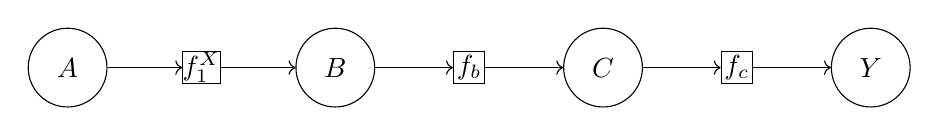
\begin{tikzpicture}[every place/.style={minimum size=10mm}, node distance=1.7cm]
  % Places
  \node[place] (A) {$A$};
  \node[transition] (fa) [right of=A] {$f_1^X$};
  \node[place] (B) [right of=fa] {$B$};
  \node[transition] (fb) [right of=B] {$f_b$};
  \node[place] (C) [right of=fb] {$C$};
  \node[transition] (fc) [right of=C] {$f_c$};
  \node[place] (Y) [right of=fc] {$Y$};

  % Arcs
  \draw[->] (A) -- (fa);
  \draw[->] (fa) -- (B);
  \draw[->] (B) -- (fb);
  \draw[->] (fb) -- (C);
  \draw[->] (C) -- (fc);
  \draw[->] (fc) -- (Y);
\end{tikzpicture}}
\caption{Resized Linear Petri Net}
\label{fig:linear_petri_resized}
\end{figure}

% Second instance as a regular figure
\begin{figure}[htbp]
\centering
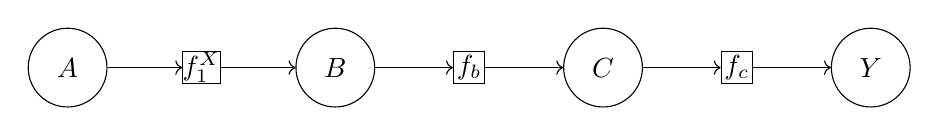
\begin{tikzpicture}[every place/.style={minimum size=10mm}, node distance=1.7cm]
  % Places
  \node[place] (A) {$A$};
  \node[transition] (fa) [right of=A] {$f_1^X$};
  \node[place] (B) [right of=fa] {$B$};
  \node[transition] (fb) [right of=B] {$f_b$};
  \node[place] (C) [right of=fb] {$C$};
  \node[transition] (fc) [right of=C] {$f_c$};
  \node[place] (Y) [right of=fc] {$Y$};

  % Arcs
  \draw[->] (A) -- (fa);
  \draw[->] (fa) -- (B);
  \draw[->] (B) -- (fb);
  \draw[->] (fb) -- (C);
  \draw[->] (C) -- (fc);
  \draw[->] (fc) -- (Y);
\end{tikzpicture}
\caption{Tensorized Petri Net Structure}
\label{fig:tensor_petri}
\end{figure}

\begin{figure}[htbp]
% Petri Net Model of the Producer-Consumer Problem (Refined)
\begin{tikzpicture}[node distance=2.2cm and 2.2cm, >=stealth, bend angle=30, auto, on grid]
    % Places
    \placewithtokens{producer}{0,0}{1}
    \placewithtokens{buffer}{2.8,0}{0}
    \placewithtokens{consumer}{5.6,0}{1}
    \placewithtokens{bufferCapacity}{2.8,-2.2}{3}

    % Transitions
    \node[transition, rounded corners=2pt] (produce) [right=of producer] {};
    \node[transition, rounded corners=2pt] (consume) [right=of buffer] {};

    % Arcs
    \draw[pre] (producer) -- (produce);
    \draw[post] (produce) -- (producer);
    \draw[post] (produce) -- (buffer);
    \draw[pre] (buffer) -- (consume);
    \draw[pre] (consumer) -- (consume);
    \draw[post] (consume) -- (consumer);
    \draw[pre] (bufferCapacity) -- (produce);
    \draw[post] (consume) -- (bufferCapacity);

    % Labels
    \node[above] at (producer.north) {Producer};
    \node[above] at (buffer.north) {Buffer};
    \node[above] at (consumer.north) {Consumer};
    \node[below] at (bufferCapacity.south) {Buffer Capacity};
    \node[above] at (produce.north) {Produce};
    \node[above] at (consume.north) {Consume};

    % Title
    \node[above=1cm] at (current bounding box.north) {Petri Net Model of the Producer-Consumer Problem};
\end{tikzpicture}
\caption{Producer-Consumer Workflow}
\label{fig:producer_consumer_workflow}
\end{figure}

\begin{figure}[htbp]
\centering
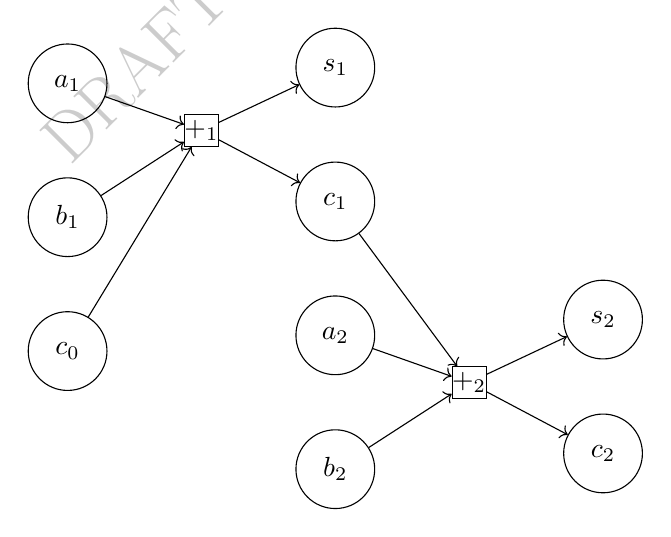
\begin{tikzpicture}[every place/.style={minimum size=10mm}, node distance=1.7cm and 2.2cm]
  % First digit addition
  \node[place] (a1) {$a_1$};
  \node[place, below of=a1] (b1) {$b_1$};
  \node[place, below of=b1] (c0) {$c_0$};
  \node[transition] (add1) [right of=b1, yshift=1.1cm] {$+_1$};
  \node[place] (s1) [right of=add1, yshift=0.8cm] {$s_1$};
  \node[place] (c1) [below of=s1] {$c_1$};

  \draw[->] (a1) -- (add1);
  \draw[->] (b1) -- (add1);
  \draw[->] (c0) -- (add1);
  \draw[->] (add1) -- (s1);
  \draw[->] (add1) -- (c1);

  % Second digit addition
  \node[place, below of=c1] (a2) {$a_2$};
  \node[place, below of=a2] (b2) {$b_2$};
  \node[transition] (add2) [right of=b2, yshift=1.1cm] {$+_2$};
  \node[place] (s2) [right of=add2, yshift=0.8cm] {$s_2$};
  \node[place] (c2) [below of=s2] {$c_2$};

  \draw[->] (a2) -- (add2);
  \draw[->] (b2) -- (add2);
  \draw[->] (c1) -- (add2);
  \draw[->] (add2) -- (s2);
  \draw[->] (add2) -- (c2);
\end{tikzpicture}
\caption{Carry Arithmetic as Feedback System.}
\label{fig:carry_arithmetic_feedback}
\end{figure}

\begin{figure}[htbp]
\centering
\resizebox{0.9\columnwidth}{!}{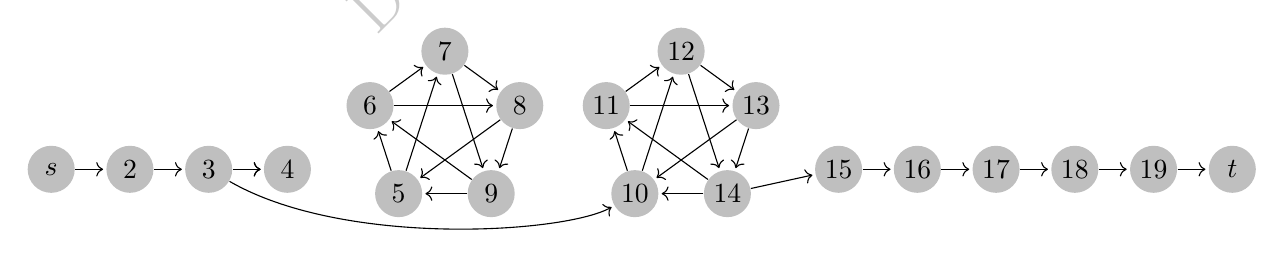
\begin{tikzpicture}
    [shorten >=1pt,->,
     vertex/.style={circle,fill=black!25,minimum size=17pt,inner sep=0pt}]
  
    \foreach \name/\x in {s/1, 2/2, 3/3, 4/4, 15/11, 16/12, 17/13, 18/14, 19/15, t/16}
      \node[vertex] (G-\name) at (\x,0) {$\name$};
  
    \foreach \name/\angle/\text in {P-1/234/5, P-2/162/6, P-3/90/7, P-4/18/8, P-5/-54/9}
      \node[vertex,xshift=6cm,yshift=.5cm] (\name) at (\angle:1cm) {$\text$};
  
    \foreach \name/\angle/\text in {Q-1/234/10, Q-2/162/11, Q-3/90/12, Q-4/18/13, Q-5/-54/14}
      \node[vertex,xshift=9cm,yshift=.5cm] (\name) at (\angle:1cm) {$\text$};
  
    \foreach \from/\to in {s/2,2/3,3/4,3/4,15/16,16/17,17/18,18/19,19/t}
      \draw (G-\from) -- (G-\to);
  
    \foreach \from/\to in {1/2,2/3,3/4,4/5,5/1,1/3,2/4,3/5,4/1,5/2}
      { \draw (P-\from) -- (P-\to); \draw (Q-\from) -- (Q-\to); }
  
    \draw (G-3) .. controls +(-30:2cm) and +(-150:1cm) .. (Q-1);
    \draw (Q-5) -- (G-15);
  \end{tikzpicture}}
\caption{Example of a complex graph structure with cycles and cross-connections.}
\label{fig:complex_graph_example}
\end{figure}

\subsection{Model Analysis}

To analyze the properties of our Petri Net model, we examine:

\begin{itemize}
    \item \textbf{Reachability}: Determining whether a specific marking can be reached from the initial marking.
    \item \textbf{Boundedness}: Ensuring that the number of tokens in each place does not exceed a finite bound.
    \item \textbf{Liveness}: Verifying that the model is free from deadlocks.
    \item \textbf{Fairness}: Ensuring that all enabled transitions eventually fire.
\end{itemize}

\subsection{Wiring Diagram Representation}

Figure \ref{fig:clock_with_display} presents a wiring diagram in the style of David Jaz Myers' work on Dynamical Systems, illustrating the structure of a clock system with display components.

\begin{figure}[htbp]
\centering
% ClockWithDisplay in Spivak/Fong style using oriented WD
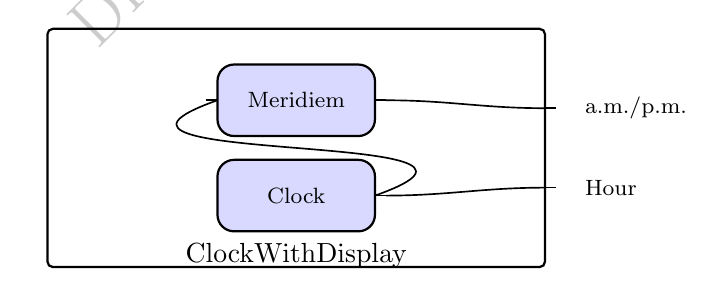
\begin{tikzpicture}[oriented WD, bbx=1.2cm, bby=2ex, bb min width=2cm, bb port length=4pt, bb port sep=1.5]
    % Clock and Meridiem boxes with proper ports and more rounded corners
    % The notation bb={in}{out} specifies number of input and output ports
    \node[bb={0}{1}, fill=blue!15, thick, rounded corners=6pt] (clock) at (0, -2) {\footnotesize Clock};
    \node[bb={1}{1}, fill=blue!15, thick, rounded corners=6pt] (meridiem) at (0, 2) {\footnotesize Meridiem};
    
    % Container box that encompasses both components with more spacing
    \node[bb={0}{2}, fit={($(clock.south west)+(-0.8,-0.5)$) ($(meridiem.north east)+(0.8,0.5)$)}, thick] (container) {};
    
    % Connection from right of Clock to left of Meridiem
    % Symmetric S-curve for Clock→Meridiem (canonical categorical style)
    \draw
      (clock.east)
      .. controls ($(clock.east)+(2,2.8)$) and ($(meridiem.west)+(-2,-2.8)$)
      .. (meridiem.west);

    
    % Connect ports to container edges for outputs
    \draw (meridiem_out1) to (container_out1');
    \draw (clock_out1) to (container_out2');
    
    % External labels with better positioning
    \node[anchor=west, font=\footnotesize] at ($(container_out1)+(0.2,0)$) {a.m./p.m.};
    \node[anchor=west, font=\footnotesize] at ($(container_out2)+(0.2,0)$) {Hour};
    
    % Title below container with better spacing
    \node[font=\normalsize] at ($(container.south)+(0,0.5)$) {ClockWithDisplay};
\end{tikzpicture}
\caption{Wiring diagram of a clock with display components, showing the meridiem and hour display units.}
\label{fig:clock_with_display}
\end{figure}

\subsection{Implementation}

[Describe the tools or methods used to implement and analyze your Petri Net model]
% \sectionheader{Results and Discussion}
\label{sec:results}

The Tensorized Petri Net formalism offers several advantages:

\begin{itemize}
    \item \textbf{Parallelism:} Tensor operations enable efficient, parallel updates of the Petri Net state, mirroring the inherent concurrency of the net.
    \item \textbf{Compositionality:} Polynomial functors provide a principled way to compose and decompose Petri Net modules, supporting scalable and reusable designs.
    \item \textbf{Interpretability:} The explicit representation of operands, operators, and their topological relationships makes the computation transparent and analyzable.
    \item \textbf{Expressiveness:} This framework generalizes naturally to other structured computations, such as cellular automata, graph algorithms, and symbolic reasoning tasks.
\end{itemize}

\subsection{Model Validation}

[Describe how you validated your Petri Net model]

\subsection{Performance Analysis}

[Present the results of your performance analysis]

\begin{table}[htbp]
\centering
\caption{Performance Metrics for Different Configurations}
\label{tab:performance}
\begin{tabular}{@{}lccc@{}}
\toprule
\textbf{Metric} & \textbf{Config 1} & \textbf{Config 2} & \textbf{Config 3} \\
\midrule
Throughput & [value] & [value] & [value] \\
Response Time & [value] & [value] & [value] \\
Resource Utilization & [value] & [value] & [value] \\
\bottomrule
\end{tabular}
\end{table}

\subsection{Case Study}

[Present a case study demonstrating the application of your Petri Net model]

\subsection{Discussion}

[Discuss the implications of your results and any limitations of your approach]

\begin{figure}[htbp]
\centering
\resizebox{0.9\columnwidth}{!}{% Petri Net Model of the Producer-Consumer Problem (Refined)
\begin{tikzpicture}[node distance=2.2cm and 2.2cm, >=stealth, bend angle=30, auto, on grid]
    % Places
    \placewithtokens{producer}{0,0}{1}
    \placewithtokens{buffer}{2.8,0}{0}
    \placewithtokens{consumer}{5.6,0}{1}
    \placewithtokens{bufferCapacity}{2.8,-2.2}{3}

    % Transitions
    \node[transition, rounded corners=2pt] (produce) [right=of producer] {};
    \node[transition, rounded corners=2pt] (consume) [right=of buffer] {};

    % Arcs
    \draw[pre] (producer) -- (produce);
    \draw[post] (produce) -- (producer);
    \draw[post] (produce) -- (buffer);
    \draw[pre] (buffer) -- (consume);
    \draw[pre] (consumer) -- (consume);
    \draw[post] (consume) -- (consumer);
    \draw[pre] (bufferCapacity) -- (produce);
    \draw[post] (consume) -- (bufferCapacity);

    % Labels
    \node[above] at (producer.north) {Producer};
    \node[above] at (buffer.north) {Buffer};
    \node[above] at (consumer.north) {Consumer};
    \node[below] at (bufferCapacity.south) {Buffer Capacity};
    \node[above] at (produce.north) {Produce};
    \node[above] at (consume.north) {Consume};

    % Title
    \node[above=1cm] at (current bounding box.north) {Petri Net Model of the Producer-Consumer Problem};
\end{tikzpicture}}
\caption{Producer-Consumer Workflow Analysis}
\label{fig:producer_consumer}
\end{figure}
% \sectionheader{Discussion}

In this section, we illustrate compositionality using wiring diagrams in the style of David Spivak.

\begin{figure*}[t]
\centering
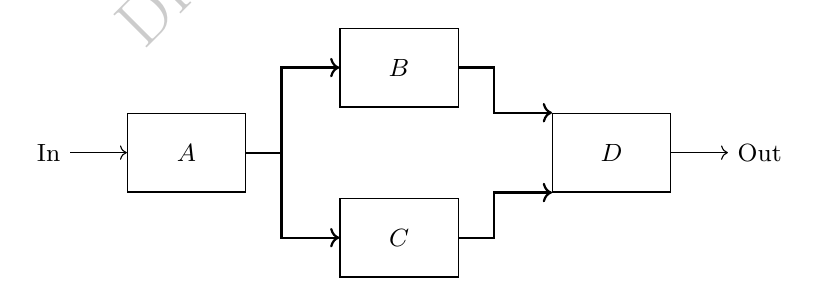
\begin{tikzpicture}[scale=0.9, every node/.style={font=\small}]
  % Boxes
  \node[draw, rectangle, minimum width=1.5cm, minimum height=1cm] (A) at (0,0) {$A$};
  \node[draw, rectangle, minimum width=1.5cm, minimum height=1cm] (B) at (3,1.2) {$B$};
  \node[draw, rectangle, minimum width=1.5cm, minimum height=1cm] (C) at (3,-1.2) {$C$};
  \node[draw, rectangle, minimum width=1.5cm, minimum height=1cm] (D) at (6,0) {$D$};

  % Wires
  \draw[->, thick] (A.east) -- ++(0.5,0) |- (B.west);
  \draw[->, thick] (A.east) -- ++(0.5,0) |- (C.west);
  \draw[->, thick] (B.east) -- ++(0.5,0) |- (D.north west);
  \draw[->, thick] (C.east) -- ++(0.5,0) |- (D.south west);

  % Inputs/Outputs
  \draw[<-] (A.west) -- ++(-0.8,0) node[left] {In};
  \draw[->] (D.east) -- ++(0.8,0) node[right] {Out};
\end{tikzpicture}
\caption{A simple wiring diagram in the style of David Spivak.}
\label{fig:wiring_diagram_1}
\end{figure*}

\begin{figure*}[t]
\centering
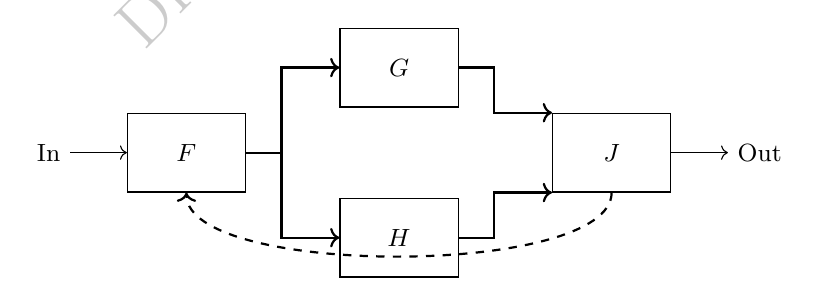
\begin{tikzpicture}[scale=0.9, every node/.style={font=\small}]
  % Boxes
  \node[draw, rectangle, minimum width=1.5cm, minimum height=1cm] (F) at (0,0) {$F$};
  \node[draw, rectangle, minimum width=1.5cm, minimum height=1cm] (G) at (3,1.2) {$G$};
  \node[draw, rectangle, minimum width=1.5cm, minimum height=1cm] (H) at (3,-1.2) {$H$};
  \node[draw, rectangle, minimum width=1.5cm, minimum height=1cm] (J) at (6,0) {$J$};

  % Wires
  \draw[->, thick] (F.east) -- ++(0.5,0) |- (G.west);
  \draw[->, thick] (F.east) -- ++(0.5,0) |- (H.west);
  \draw[->, thick] (G.east) -- ++(0.5,0) |- (J.north west);
  \draw[->, thick] (H.east) -- ++(0.5,0) |- (J.south west);

  % Feedback wire
  \draw[->, thick, dashed] (J.south) .. controls +(0,-1.2) and +(0,-1.2) .. (F.south);

  % Inputs/Outputs
  \draw[<-] (F.west) -- ++(-0.8,0) node[left] {In};
  \draw[->] (J.east) -- ++(0.8,0) node[right] {Out};
\end{tikzpicture}
\caption{A wiring diagram with feedback, inspired by David Spivak's style.}
\label{fig:wiring_diagram_2}
\end{figure*}

% Bibliography
\nocite{*}

% Custom bibliography formatting for better wrapping of long references
\makeatletter
\def\url@leostyle{\@ifundefined{selectfont}{\def\UrlFont{\sf}}{\def\UrlFont{\small\ttfamily}}}
\makeatother
\urlstyle{leo}

% Adjust the maximum width for URLs in bibliography
\Urlmuskip=0mu plus 3mu

% Add more flexibility to where LaTeX can break lines in bibliography
\sloppy
\emergencystretch=2em

% Use IEEEtran style with our custom settings
\bibliographystyle{IEEEtran}
\bibliography{bibliography}

\end{document}
